\documentclass[fleqn, twocolumn, 10pt]{article}
\usepackage{afterpage}
\usepackage{graphicx}
\usepackage{amsmath, bm}
\usepackage{centernot}
\usepackage{mathtools}
\usepackage{stmaryrd}
\usepackage{wrapfig}
\usepackage[sort&compress]{natbib}
\usepackage{tikz}
\usepackage{ctable}
\usepackage{amssymb}
\usepackage{caption}
\usepackage{amstext}
\usepackage[greek,english]{babel}
\usepackage{amsmath}
\usepackage[utf8]{inputenc}
\usepackage{fancyhdr}
\usepackage{caption}
\usepackage[margin=0.6in]{geometry}
\usepackage{titlesec}
\usepackage{eucal}
\usepackage{upgreek}
\usepackage{nccmath}
\usetikzlibrary{shapes.geometric}
\usetikzlibrary{shapes.misc}
\newcommand{\hookuparrow}{\mathrel{\rotatebox[origin=c]{90}{$\hookrightarrow$}}}
\newcommand{\hookdownarrow}{\mathrel{\rotatebox[origin=c]{-90}{$\hookrightarrow$}}}
\hyphenpenalty=10000
\captionsetup[figure]{font=footnotesize}
\newcommand{\changefont}{\fontsize{9}{10}\selectfont}
\pagestyle{fancy}
\fancyhf{}
\rhead[LE,RO]{\changefont \slshape Final Report}
\lhead[RE,LO]{\changefont \slshape The Search for Magnetic Monopoles}
\cfoot{\thepage}
\renewcommand{\headrulewidth}{2pt}
\renewcommand{\footrulewidth}{1pt}
\usepackage{titling}
\renewcommand\maketitlehooka{\null\mbox{}\vfill}
\renewcommand\maketitlehookd{\vfill\null}
\tikzset{cross/.style={cross out, draw=black, minimum size=2*(#1-\pgflinewidth), inner sep=0pt, outer sep=0pt}, cross/.default={3pt}}
\setcounter{secnumdepth}{4}
\titleformat{\paragraph}
{\normalfont\normalsize\bfseries}{\theparagraph}{1em}{}
\titlespacing*{\paragraph}
{0pt}{3.25ex plus 1ex minus .2ex}{1.5ex plus .2ex}
\setlength{\mathindent}{0pt}
\renewcommand{\arraystretch}{1.3}
\newcommand {\scalelinespace} [1] {\rule{0pt}{#1\normalbaselineskip}}

\begin{document}
\captionsetup[figure]{labelfont={bf},name={Fig.},labelsep=period}
%TITLE PAGE%%%%%%%%%%%%%%%%%%%%%%%%%%%%%%%%%%%%%%%%%%%%%%%%%%
\begin{titlepage}
	
	\centering
	\vspace*{1cm}
	{\scshape\LARGE University of Leeds \par}
	\vspace{0.5cm}
	\begin{figure}[h]
	\centering
	
\includegraphics[width=30mm,scale=0.2]{University_of_Leeds_crest.png}
	\end{figure}
	\vspace{1cm}
	\begin{tabular}{ccc}
	\specialrule{.05em}{.1em}{.1em}
	\specialrule{.3em}{.2em}{.2em}\\
	{\scshape\large FINAL YEAR PROJECT\par}\\
	\vspace{1cm}\\
	{\huge\bfseries The Search for Magnetic Monopoles\par}\\
	\vspace{1cm}\\
	{\Large\itshape\bfseries James Ovenden\par}\\
	\vspace{0cm}\\
	\specialrule{.3em}{.2em}{.2em}
	\specialrule{.05em}{.1em}{.0em}\\
	\vspace{0.5cm}\\
	{\scshape\large CHARGE QUANTISATION, TOPOLOGICAL FORMALISM AND}\\
	{\scshape\large RESULTS FROM GEOMETRY\par}
	\end{tabular}
	
	\vfill
	Supervisor---\par
	Dr~Robert \textsc{Purdy}\\
	\vspace{1cm}
	Assessor---\par
	Prof.~Ben \textsc{Varcoe}\\
	\vspace{1cm}
	{\scshape\large \textnormal{Submitted in accordance with the requirements for a research project\\ for the degree of}}\\
	{\scshape\large \textit{Combined Bachelor of Science and Master of Physics} \par}
	\vfill
	{\large \today\par}
\end{titlepage}

% DECLARATION %%%%%%%%%%%%%%%%%%%%%%%%%%%%%%%%%%%%%%%%%%%%%%%%%%
\thispagestyle{plain}
\font\myfont=cmr12 at 20pt
\newgeometry{margin=1.5in}
\onecolumn
\fontsize{11}{14}\selectfont
\section*{\centering \huge Declaration}
\vspace{0.75cm}
I can hereby certify that any work in this thesis that is not my own has been properly acknowledged and cited.
\newpage
\clearpage


% ACKNOWLEDGEMENTS %%%%%%%%%%%%%%%%%%%%%%%%%%%%%%%%%%%%%%%%%%%%%%%%%%
\thispagestyle{plain}
\onecolumn
\section*{\centering \huge Acknowledgements}
\vspace{0.75cm}
I would like to thank Dr Robert Purdy for his continued support in my preparation for this project report. I would also like to thank Prof. Ben Varcoe as my assessor along with the rest of the staff in the Theoretical Physics group from the Physics and Astronomy department at the University of Leeds. Finally, I want to extend this acknowledgement to my family and friends who for many years tried to listen to, and comprehend, my spectacular physics and maths-related digressions. May whoever views this piece gain as much enjoyment from reading it as I did writing it.
\clearpage

% ABSTRACT %%%%%%%%%%%%%%%%%%%%%%%%%%%%%%%%%%%%%%%%%%%%%%%%%%

\thispagestyle{plain}
\onecolumn
\section*{\centering \huge Abstract}
\vspace{0.75cm}
The magnetic monopole is and has been the subject of many a physicist's entire career. Its discovery would help us paint the mathematical picture of the Universe we live in due to its sheer prevalence in `Grand Unified Theories' (GUTs). It would also give us a fundamental reason for the quantisation of electric charge and help to confirm one of the most radical, but now widely accepted, concepts in cosmology. This paper aims to present these ideas in more detail before looking at the geometrical and topological origin of the Dirac monopole, and why its charge is deemed, itself, `topological' in comparison to the `non-topological' electric charge. There is also a means to give further insight into the application of such maths in the realm of electrodynamics.
\clearpage
\fontsize{11}{15}\selectfont
\thispagestyle{plain}
\tableofcontents
\thispagestyle{plain}
\clearpage
\restoregeometry
%%%%%%%%%%%%%%%%%%%%%%%%%%%%%%%%%%%%%%%%%%%%%%%%%%%%%%%%%%
% REPORT %%%%%%%%%%%%%%%%%%%%%%%%%%%%%%%%%%%%%%%%%%%%%%%%%%%%%%%%%%%%%%%%%%%%%%%%%%%%%%%%%%%%%%%%%%%%%%%%%%%%%%%%%
\fontsize{10}{12}\selectfont
\section{Introduction}

The field of science has taught many to think critically of results and look beyond what one may observe in experiments. Such thirst for knowledge has seen the human race grow and thrive in its relatively short existence. Theoretical Physics takes the next step: to predict observation. Using mathematics to model the entirety of nature is the ultimate aim for many; to reduce the rules of the universe to a set of axioms, constants and equations. Unfortunately, to verify such a `Theory of Everything' (ToE), predictions must align with experiment and observation. One such prediction of many a ToE and all GUTs is that of the existence of the magnetic point charge.

This paper aims to look at the motivations behind studying this particle and some of the reasons to support its existence in section 2 before looking at the maths behind---in the lead up to the formulation of---the Dirac monopole. Specifically, this piece will give the mathematical reasoning behind the \textit{topological} nature of the magnetic charge of this monopole. In doing this, it will also be able to address the contrasting \textit{non-topological} nature of electric charge. This paper will also look to present other monopole-related topics in which such concepts are useful: like in the realm of quantum field theory. 

The Dirac monopole is best described using \textit{fibre bundles}, and this piece will serve to provide the reader with the tools to understand how such mathematical structures are formalised and applied in the case of electrodynamics. This will be done through first looking at calculus on manifolds, before applying that to the context of Lie groups. In reading about fibre bundles, readers should gain insight into why principal bundles are most appropriate for gauge theories, and why the Hopf bundle is applicable here. Finally, characteristic classes will be able to show how \textit{characteristics} of bundles can be obtained and how they relate to the physical world.

%%%%%%%%%%%%%%%%%%%%%%%%%%%%%%%%%%%%%%%%%%%%%%%%%%%%%%%%%%
% MOTIVATIONS %%%%%%%%%%%%%%%%%%%%%%%%%%%%%%%%%%%%%%%%%%%%%%%%%%%%%%%%%%%%%%%%%%%%%%%%%%%%%%%%%%%%%%%%%%%%%%%%%%%%%%%%%

\section{Motivations}

Emmy Noether showed us that nature and symmetry are intrinsically linked on the physical level using Lagrangian mechanics. She theorised that for a particular continuous symmetry in a particle's Lagrangian, there is an associated conserved quantity \cite{bob2017purdy}. Noether's theorem is widely considered to be one of the most beautiful results of mathematics and \textit{`a guiding star to 20th and 21st-century physics'} according to Professor Frank Wilczek of MIT \cite{scinews}. It is the human condition to continue to search for such satisfying and beautiful phenomena in the Universe and this elegance in physics doesn't end there; another such example comes in the form of Maxwell's equations.

\subsection{Symmetry in Maxwell's equations}
James Clerk Maxwell formulated his equations in 1861 and developed the symmetry between electricity and magnetism \cite{maxwell1861li}. It can be easily seen, even with the presence of arbitrary constants, that both the electric and magnetic fields are almost indistinguishable in the absence of a source 

\begin{ceqn}
\begin{align*}
\nabla \cdotp \mathbf{E} = 0   \ \ \text{(1.1a)} \ \ \ \nabla \times \mathbf{E} = \frac{-1}{c}\frac{\partial \mathbf{B}}{\partial t} \ \  \text{(1.1b)}
\end{align*}
\end{ceqn}
\begin{ceqn}
\begin{align*}
\nabla \cdotp \mathbf{B} = 0   \ \ \text{(1.1c)} \ \ \ \nabla \times \mathbf{B} = \frac{1}{c} \frac{\partial \mathbf{E}}{\partial t} \ \ \text{(1.1d)}
\end{align*}
\end{ceqn}
where Gaussian unit convention is used. Introducing an electric charge and current into the system, the equations become \cite{maxwell1861li, martin2015phys}
\begin{ceqn}
\begin{align*}
\nabla \cdotp \mathbf{E} = 4\pi\rho \ \ \text{(1.2a)} \ \ \nabla \times \mathbf{E} = \frac{-1}{c}\frac{\partial \mathbf{B}}{\partial t} \ \ \ \text{(1.2b)}
\end{align*}
\end{ceqn}
\begin{ceqn}
\begin{align*}
\nabla \cdotp \mathbf{B} = 0   \ \ \text{(1.2c)} \ \ \ \nabla \times \mathbf{B} = \frac{1}{c}\left(4\pi\mathbf{J} + \frac{\partial \mathbf{E}}{\partial t}\right) \ \ \text{(1.2d)}\text{.} 
\end{align*}
\end{ceqn}
Though still beautiful, this offers an unsatisfying result. The symmetry between $\mathbf{E}$ and $\mathbf{B}$ is lost. So far, though, only an electric point charge is present in the system. When a magnetic point source is introduced, Maxwell's equations take the form \cite{ellismagnetic}
\begin{ceqn}
\begin{align*}
\nabla \cdotp \mathbf{E} = 4\pi\rho  \ \ \text{(1.3a)} \ \ \ \nabla \times \mathbf{E} = \frac{-1}{c}\left(\frac{\partial \mathbf{B}}{\partial t} + 4\pi\mathbf{J}_{m}\right) \ \  \text{(1.3b)}
\end{align*}
\end{ceqn}
\begin{ceqn}
\begin{align*}
\nabla \cdotp \mathbf{B} = 4\pi\rho_{m}  \ \ \text{(1.3c)} \ \ \ \nabla \times \mathbf{B} = \frac{1}{c}\left(\frac{\partial \mathbf{E}}{\partial t} + 4\pi\mathbf{J}\right) \ \ \text{(1.3d)}   
\end{align*}
\end{ceqn}
with $\rho_{m}$ and $\mathbf{J}_{m}$ being magnetic charge density and current respectively. The symmetry has been restored! The magnetic monopole provides a wonderful solution to this symmetry `problem'. Even without observation of a monopole, as Paul Dirac once wrote---\textit{`one would be surprised if nature made no use of it'} \cite{dirac1931quantised, arcidiacono1978tachyons}.

% CHARGE QUANTISATION %%%%%%%%%%%%%%%%%%%%%%%%%%%%%%%%%%%%%%%%%%

\subsection{Electric Charge Quantisation}

Philosophical physicists might posit the question of why the Universe possesses the particular characteristics we observe. This is a question that we may never be able to answer fully; we could be seeing most things in the Universe merely because that is how our universe behaves (we also can't compare to any others!). Considerations of massless gauge fields gave a solution to an example of such phenomena---the quantisation of electric charge---in 1974 \cite{georgi1974unity}. It was in 1931, though, that Paul Dirac first offered a reason behind the discreteness of the electron using the existence of a magnetic point source. 

The charge quantisation condition can be proven using T.T. Wu's and C.N. Yang's approach who constructed a theory of an Abelian monopole in 1975 \cite{WuMonopoleYang}, but first, a revisit to Dirac's 1931 paper is required. Dirac postulated the idea of a string, a one-dimensional singularity analogous to an infinitely thin solenoid, that ended with a monopole. They are unobservable and lead to an unpleasant proof but can be eliminated using the Wu-Yang monopole method. With the presence of a Dirac string, a global potential cannot exist as it will be undefined on this singularity. To mitigate this issue, two hemispherical coverings, $\mathbf{R^n}$ and $\mathbf{R^s}$, are defined with identical radii and respective potentials $\mathbf{A^n}$ and $\mathbf{A^s}$. Being a non-singular theory, one must remove the monopole---as it is, itself, a singularity---from the origin, along with the string. So, therefore, only consider the $\mathbb{R}^3$\textbackslash\{$0$\} space.\\

\begin{figure}[t]
\centering
\begin{tikzpicture}
\shade[ball color = grey!40, opacity = 0.4] (0,0) circle (4cm);
\draw (0,0) circle (4cm);
\draw[dashed] (4,0.05) arc (0:360:4 and 2);
\draw[dashed] (4,-0.05) arc (0:360:4 and 2);
\fill[fill=black] (0,0) circle (1pt);
\draw[ ->, >=stealth] (0,0 ) -- node[below]{$Y$} (5,0);
\draw[ ->, >=stealth] (0,0 ) -- node[left]{$Z$} (0,5);
\draw[ ->, >=stealth] (0,0 ) -- node[left]{$X$} (-2.5,-4.5);
\draw[very thick, ->, >=stealth] (-2.5,-0.93) -- node[left]{$\bm{\varepsilon}$} (-2.5,-1.51);
\node (a) at (1,3) {$\mathbf{R^n}$};
\node (b) at (1,-3) {$\mathbf{R^s}$};
\node (c) at (-0.5,0) {$g$};
\draw[very thick, ->, >=stealth] (-2.5,-2.19) -- node[left]{$$} (-2.5,-1.61);
\shade[ball color = black!40] (0,0) circle (0.1cm);
\end{tikzpicture}
\caption{Two overlapping hemispheres, $\mathbf{R^n}$ and $\mathbf{R^s}$, in $\mathbb{R}^3$. Removing singularity $\bm{g}$ would give this arrangement in the $\mathbb{R}^3$\textbackslash \{$0$\} space.}
\end{figure}

\indent One can now quantify the potentials in these regions

\begin{ceqn}
\begin{align*}
\mathbf{A^n} = \bm{g}\frac{1 - \cos\theta}{r\sin\theta}\hat\phi \ \ \ \ \ \ \ \ 0 \leq \theta < \frac{\pi}{2} + \frac{\bm{\varepsilon}}{2}
\end{align*}
\end{ceqn}
\begin{ceqn}
\begin{align*}
\mathbf{A^s} = -\bm{g}\frac{1 + \cos\theta}{r\sin\theta}\hat\phi \ \ \ \ \ \ \ \ \frac{\pi}{2} - \frac{\bm{\varepsilon}}{2} < \theta \leq 0
\end{align*}
\end{ceqn}
where $\bm{g}$ is the magnetic charge and $r$ the radius of the hemispheres. With the string lying along the $z$-axis, the coverings have ensured that it is also effectively removed from the system. The limits on $\theta$ that allow the string to be excluded are $\theta = \pi$ in $\mathbf{R^n}$ and $\theta = 0$ in $\mathbf{R^s}$. It can also be seen from Fig.~1 that the area of overlap, $\bm{\varepsilon}$, is infinitesimal and equal to $\mathbf{R^n}\cap\mathbf{R^s}$. 

Although these hemispheres contain two different potentials,  they encompass the same magnetic field. Using this fact and equation (1.2c) it can be shown that $\mathbf{B} = \nabla\times\mathbf{A^n} = \nabla\times\mathbf{A^s}$. It also follows that $\mathbf{A^n}$ and $\mathbf{A^s}$ are related with a gauge transformation in $\bm{\varepsilon}$ where, as previously mentioned, $\bm{\varepsilon}=\mathbf{R^n}\cap\mathbf{R^s}$. Thus the limits of $\theta$ for this region can be defined: $\frac{\pi}{2} - \frac{\bm{\varepsilon}}{2} < \theta < \frac{\pi}{2} + \frac{\bm{\varepsilon}}{2}$. Now a gauge function can be deduced using the difference in these potentials in region $\bm{\varepsilon}$:

\begin{ceqn}
\begin{align*}
\mathbf{A^n}-\mathbf{A^s}=\frac{2\bm{g}\hat\phi}{r\sin\theta}=\frac{2\bm{g}\hat\phi}{r\sin(\frac{\pi}{2}\pm\frac{\bm{\varepsilon}}{2})}=\frac{2\bm{g}\hat\phi}{r}
\end{align*}
\end{ceqn}
as $\bm{\varepsilon}\longrightarrow0$, and thus

\begin{ceqn}
\begin{align*}
\frac{2\bm{g}\hat\phi}{r} = \nabla(2\bm{g}\phi) = \nabla\bm{\Lambda}
\end{align*}
\end{ceqn}
where $\bm{\Lambda}$ is a newly defined gauge function: $\bm{\Lambda} = 2\bm{g}\phi$.

It is at this point where an electric point charge is introduced. Two wavefunctions are required here: $\bm{\psi}^n$ in $\bm{R}^n$ and $\bm{\psi}^s$ in $\bm{R}^s$. If this charge lies within the region $\bm{\varepsilon}$, the aforementioned wavefunctions must be related by a phase transformation of the form

\begin{ceqn}
\begin{align*}
\bm{\psi}^n = \bm{e}^\frac{iq\bm{\Lambda}}{\hbar c}\bm{\psi}^s = \bm{e}^\frac{iq\bm{2\bm{g}\phi}}{\hbar c}\bm{\psi}^s.
\end{align*}
\end{ceqn}
A wavefunction can only have one value at a single point, so allowing the electric charge to traverse $2\pi$ around the sphere within $\bm{\varepsilon}$ (the $x$-$y$ plane) will yield the same value. This leads to the case that $\bm{\psi}^n|_\phi = \bm{\psi}^n|_{\phi+2\pi}$. It can now be deduced that 

\begin{ceqn}
\begin{align*}
\bm{\psi}^n = \bm{e}^\frac{iq\bm{2\bm{g}\phi}}{\hbar c}\bm{\psi}^s = \bm{e}^\frac{iq\bm{2\bm{g}(\phi+2\pi)}}{\hbar c}\bm{\psi}^s
\end{align*}
\end{ceqn}
and so

\begin{ceqn}
\begin{align*}
\bm{e}^\frac{iq\bm{2\bm{g}\phi}}{\hbar c} = \bm{e}^\frac{iq\bm{2\bm{g}(\phi+2\pi)}}{\hbar c}
\end{align*}
\end{ceqn}
which leads to

\begin{ceqn}
\begin{align*}
\bm{e}^\frac{iq\bm{g}4\pi}{\hbar c} = 1.
\end{align*}
\end{ceqn}
From this, it is now clear that 

\begin{ceqn}
\begin{align*}
q\bm{g} = \frac{n\hbar c}{2}.
\end{align*}
\end{ceqn}

A wavefunction will indeed expand to every point in the universe (at the speed of light $c$, of course), even if such a wavefunction would be immeasurably weak at large distances. Thus this wonderfully elegant proof shows that the presence of a magnetic monopole at any point in the Universe would give a reason for the quantised nature of electric charge and, as such, provides a huge reason to speculate its existence. Such an arrangement will be returned to when looking at the Hopf map in section 7.1, and when addressing the origin of magnetic charge in section 8 \cite{Heras_2018, shnir, preskill1984magnetic}.

% HIGGS-GAUGE FIELD COUPLING %%%%%%%%%%%%%%%%%%%%%%%%%%%%%%%%%%%%%

\subsection{Higgs-EM Field Coupling and The Magnetic Conclusion}

Later in this paper, in section 6, gauge fields and Lie groups will be discussed. These topics are of great importance in quantum field theory and provide foundations for many a GUT. Fields don't just exist independently, though, and interactions between fields need to be considered when attempting to formalise a GUT. The group $SU(2)$ is a Lie group, and it will be seen that the coupling between this $SU(2)$ \textit{gauge field} and the Higgs field helps to describe the magnetic nature of a type of monopole that bears many similarities to that of Dirac's: the 't~Hooft-Polyakov monopole. For now, though, and to help illustrate why coupling between fields is such an important concept, consider the following example.

\subsubsection{A Theory Without Coupling}

Define a sphere of radius $r$ in the Higgs field with the 't~Hooft Polyakov monopole at the centre. The potential energy associated with the Higgs field $\phi$ within this sphere is

\begin{ceqn}
\begin{align*}
E_{Higgs} = 4\pi \int (\nabla\phi)^2 r^2 dr.
\end{align*}
\end{ceqn}
When near to the defect, calculating $\nabla\phi$ can be quite complicated. Far away, though, the gradient of the Higgs field varies with the inverse of the radius. This gives an integral of the form

\begin{ceqn}
\begin{align*}
E_{Higgs} = 4\pi \int \left(\frac{1}{r}\right)^2 r^2 dr = 4\pi r.
\end{align*}
\end{ceqn}

As previously mentioned, the defect is a 0-dimensional singularity; a point in space-time (and thus, in the Higgs field). One could, therefore, be forgiven for questioning this result, which suggests that the energy diverges with the radius of the sphere. As previously indicated, though, this example only considers energy in the Higgs field. Section 6 will outline where coupling involving the Higgs field comes in and will cover such ideas in more detail.


% MONOPOLE PROBLEM %%%%%%%%%%%%%%%%%%%%%%%%%%%%%%%%%%%%%%%%%%%

\subsection{The Magnetic Monopole Problem}

It turns out that the concept of the magnetic monopole plays a large part in our understanding of how the Universe behaved in its very early stages. A now widely accepted theory of the Universe’s inception uses the idea of inflation and was presented by Alan Guth in 1981 \cite{preskill1984magnetic, liddle2015cosmo, guth1981inflate, Ian2002Lawrie}, but it was another of his papers published a year prior that explored the importance of the magnetic monopole.

\subsubsection{Monopole Production in the Early Universe}

The early Universe is thought to have been incredibly hot but it was also cooling at a rapid rate. Eventually, the temperature would be such that spontaneous symmetry breaking could occur in the Higgs field, at around $10^{15}$ GeV. Guth proposed the idea of entities called `bubbles'. These would develop from a phase transition at a single point with a particular Higgs field value. A bubble greater than a critical size would expand with surrounding areas of the field to falling into the same configuration, giving them the same value. One can visualise this as being analogous to a growing crystalline structure.
\begin{figure}[h!]
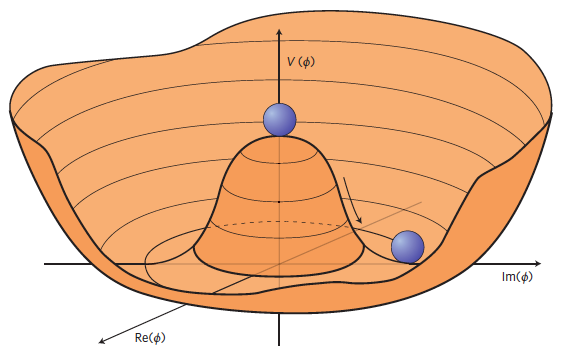
\includegraphics[width=\linewidth]{higgspotential.png}
\caption{`Mexican hat' Higgs potential. One can see that values in the field are determined randomly when symmetry is broken \cite{Ellis_2016}.}
\end{figure}

\subsubsection{From Bubbles to Monopoles}
Bubbles could lead to the production of a monopole in different ways, but the easiest to visualise and the first presented by Guth was the idea of `bubble coalescence'. This would involve two separate bubbles, both initially out of causal contact with each other, growing and eventually coming into contact. These bubbles would most likely have different values in the Higgs field, and so to extrapolate on the crystal analogy: they would have differing orientations. The field would then attempt to align itself, conserving as much energy as possible between these different orientations. The result is a topological defect or \textit{knot}; this knot would later be known as an 't~Hooft-Polyakov magnetic monopole \cite{guth1980early, tHooft1974gauge, polyakov1996particle}.
\begin{figure}[h]
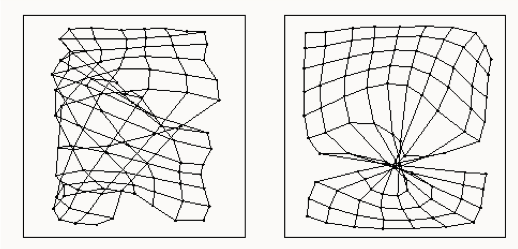
\includegraphics[width=\linewidth]{Topological_defect.png}
\caption{`Topological defects of a two-dimensional network: left folding, right twist'---Visualisation of a knot in the Higgs field \cite{topological2005defect}.}
\end{figure}

% KIBBLES FORMALISM %%%%%%%%%%%%%%%%%%%%%%%%%%%%%%%%%%%%%%%%%%%%

\subsubsection{Kibble's Formalism} 
With the temperatures lowering, it is statistically likely that many regions of the Higgs field will eventually have their symmetry broken. Thomas Kibble showed that one can assume one monopole per causally connected region of the Higgs field \cite{kolb1990early, arrtu2013conf}. This allows for a calculation of the monopole number density. 
The minimum distance at which two areas are out of causal contact with each other is defined to be $\zeta$. There is also a near-negligible probability $p_{monopole}$ associated with the production of a monopole which takes into account monopole-antimonopole annihilation. This gives a monopole density in the phase transition of \cite{preskill1984magnetic, shi2013diss}

\begin{ceqn}
\begin{align*}
n_{monopole} = \frac{p_{monopole}}{\zeta^{3}}.
\end{align*}
\end{ceqn}

It is difficult to compute an exact value for $\zeta$ but, using the concept of the particle horizon, it can be narrowed down. The particle horizon will be the shortest distance that is out of causal contact with an observer, so this must be the upper bound

\begin{ceqn}
\begin{align*}
\zeta < r_H.
\end{align*}
\end{ceqn}
This also gives a lower bound on the monopole density

\begin{ceqn}
\begin{align*}
n_{monopole} = \frac{p_{monopole}}{r_H^3}.
\end{align*}
\end{ceqn}

\subsubsection{Scale Factor, Density and Time due to Monopoles}

GUT symmetry breaking is believed to have occurred at $t_{GUT}\approx10^{-36}$\:s. Taking this to be the moment of creation for all monopoles, it is found that

\begin{ceqn}
\begin{align*}
n_{monopole,t_{GUT}} = \frac{p_{monopole}}{(2ct_{GUT})^3} \approx 10^{81}.
\end{align*}
\end{ceqn}
To calculate the ratio of the Universe's scale factor, $\bm{a}$, between $t_{GUT}$ and now, consider that $\rho_{rad} \propto \bm{a}^{-4}$. Treating the Universe as a perfect blackbody, this gives the result $T \propto \bm{a}^{-1}$ and yields a value for $\bm{a}$ of the form \cite{liddle2015cosmo}

\begin{ceqn}
\begin{align*}
\bm{a}_{t_{GUT}} = \frac{T_{CMB}}{T_{GUT}} = \frac{T_{CMB}k_B}{10^{15}GeV} \approx 10^{-29}.
\end{align*}
\end{ceqn}

Matter varies as $\rho_{mat} \propto \bm{a}^{-3}$, this would result in a current monopole density of

\begin{ceqn}
\begin{align*}
n_{m,t_{0}} = \frac{n_{m,t_{GUT}}}{{\bm{a}_{t_{GUT}}^3}}= \frac{10^{82}}{(10^{-29})^{-3}} \approx 1 \text{ monopole } m^{-3}
\end{align*}
\end{ceqn}
where $n_{m,t_{0}} = n_{monopole,t_{now}}$. The mass of a magnetic monopole turns out to be approximately $\frac{1}{\alpha}$ times the scale of GUT symmetry breaking where $\alpha$ is the fine structure constant of electrodynamics ($\approx\frac{1}{137}$) \cite{guth2015lecs}. This gives the monopole a staggering mass of around $10^{17}$ GeV$c^{-2}$ or $0.2 \mu g$! Mass density due to monopoles is thus found to be $\rho_m = 0.2\times10^{-9}\; kgm^{-3}$. This value can now be used to calculate the age of the Universe merely due to magnetic monopoles. One can start with the density parameter $\Omega(t)$

\begin{ceqn}
\begin{align*}
\Omega(t) = \frac{\rho_m}{\rho_c}
\end{align*}
\end{ceqn}
where $\rho_c$ is the critical density of the Universe \cite{liddle2015cosmo}. Finally, the equation \cite{guth2015lecs}

\begin{ceqn}
\begin{align*}
t = \frac{\pi}{2H\sqrt\Omega}
\end{align*}
\end{ceqn}
gives an upper bound on time of 206 years. 

After careful consideration, one might suggest that this is, in fact, not the age of the Universe. This is the crux of the magnetic monopole problem, and it supports one of the most radical ideas in cosmology. \\
\indent A now widely accepted theory of the Universe's inception used the idea of inflation and was presented by Alan Guth in 1981. Guth proposed that two problems---the horizon and flatness problems---could be nullified if the early Universe underwent a period of rapid inflation. Inflation is defined as the accelerating expansion of the universe or $\bm{\ddot{a}} > 0$, whereby 1$m^3$ of the Universe pre-inflation would increase to around $10^{43}m^3$ in around $10^{-34}$s \cite{liddle2015cosmo}(some inflationary models even predict a staggering scale factor of $10^{10^8}$). This is about the size of the observable Universe! Whilst Guth was investigating the problem of present-day monopole numbers (or lack thereof), he found that the appropriate characteristics of the false vacuum state would `force one into the inflationary scenario' \cite{guth1981inflate}. It seemed---rather ironically---that the magnetic monopole problem had created its own solution. This solution was able to solve the horizon and flatness problems, whilst `inflating away' the monopoles \cite{liddle2015cosmo, rajantie2012magnetic} along with any other `relic particles'. Astonishingly, it would also suggest that there may be only a single monopole in our region of the cosmos from its inception. 

%%%%%%%%%%%%%%%%%%%%%%%%%%%%%%%%%%%%%%%%%%%%%%%%%%%%%%%%%%
% PRELIM MATHS %%%%%%%%%%%%%%%%%%%%%%%%%%%%%%%%%%%%%%%%%%%%%%%%%%%%%%%%%%%%%%%%%%%%%%%%%%%%%%%%%%%%%%%%%%%%%%%%%%%%%%%%%

\section{\mbox{Monopole Formalism: Preliminary} Mathematics}

Topology may be deemed by many to have first been applied to Physics by Poincar\'e in 1890, whilst looking at solutions in celestial mechanics as curves on manifolds \cite{simon2018tying}. Topological physics provides huge areas of study today, with it and geometry underpinning some of the most prestigious theories in all of science. Maths in these areas provided new insight into formulations of physical theories; such as Maxwell formulating a theory of electromagnetism with the application of Fibre Bundles, or Riemannian geometry providing the groundwork for Einstein’s General Relativity \cite{papic2020powerpoint}. Now the two fields are so intrinsically linked that it can be deemed a two-way street---rather, the physics can give rise to new mathematical techniques. This has been seen as recently as August 2019 with work on the behaviour of neutrinos \cite{neutrino2019eigenvalues} but evidence of this is also prevalent in theories such as string theory.

The following sections take a look at the topological and geometrical formulations of electromagnetism. Differential forms, Lie groups and gauge theories will then aid in the study of the magnetic nature of the 't~Hooft-Polyakov monopole. First, there will be looks at homeomorphisms and homotopy groups before building on that with differentiable manifolds. The formalism of the Dirac monopole will become much clearer when looking at fibre bundles, and connections on fibre bundles. The general convention with these parts will be to explain a concept and then offer a more mathematically rigorous justification. 

% HOMEOMORPHISMS %%%%%%%%%%%%%%%%%%%%%%%%%%%%%%%%%%%%%%%%%%%%

\subsection{Homeomorphisms}
Two objects are deemed to be homeomorphic if they can be continuously deformed into each other. One can imagine two separate pieces of string both fixed at their ends; they can be seen as ‘paths’. While they may have differing configurations initially, they can merely be pushed (deformed) into the same configuration such that the shape of their paths is indistinguishable. This idea can be applied to many different types of objects in topology, and keen readers may have heard of the idea that a doughnut (or, rather, a torus) can be deformed into a coffee mug. This is due to the homeomorphism between the two shapes. 

More specifically, one can imagine two topological spaces U and V. U and V are homeomorphic, often denoted as $U\cong V$, if there is a continuous bijective map $f: U\to V$ with an inverse $f^{-1}: V\to U$ which is also bijective and continuous. The map $f$ is said to be the homeomorphism between $U$ and $V$. A homeomorphism is an equivalence relation. This means that one can form subsets on a topological structure according to whether it is possible to deform one space into another via a homeomorphism. Properties of a topological system that are conserved here are called \textit{topological invariants} \cite{nakahara2003geometry, sharp2019topology, zirnbauer2013topology, korner2015metric, kobayashi1963foundations}.

% HOMOTOPIES %%%%%%%%%%%%%%%%%%%%%%%%%%%%%%%%%%%%%%%%%%%%%%%

\subsection{Homotopies and Homotopy Groups}
Homotopies are intrinsically linked to homeomorphisms, but expand upon the topic; homotopies concern the continuous deformation of maps from one to another. Let $X$ and $Y$ be topological spaces and let $\mathfrak{F}$ denote the set of continuous maps from $X$ to $Y$. Given two maps $g,h \in \mathfrak{F}$, if $g(X)$ can be continuously deformed into $h(X)$ in $Y$, one can define an equivalence relation $\sim$ in $\mathfrak{F}$ between the two. This equivalence relation can be referenced by suggesting that $g$ is \textit{homotopic to} $h$. Elements that are homotopic to each other are part of the same homotopy class.

To get more of a grasp on the topic, define the set of maps $\mathfrak{A}$ that map a line, or interval $I = [0,1] \in \mathbb{R}$ to a topological surface $X$. This gives $f: I \to X$ for any $f \in \mathfrak{A}$. Take $f,j \in \mathfrak{A}$ and let $X = D^2\backslash\{0\}$, where $D^2$ denotes a two-disc (so $X$ is essentially a ring). One can imagine two lines traversing from the right to the left within this ring, where one line passes underneath the hole and the other over. However one might try, it is impossible to deform these lines into each other. Thus they aren't homotopic and neither are they part of the same homotopy class.

This idea can be extrapolated to loops; loops can be divided into homotopy classes associated with how many times $n$ they encircle a hole, this is referred to as the \textit{winding number}. It is worth noting that the direction of this \textit{winding} is also taken into consideration.

The set of homotopy classes has a group structure by nature, which gives the fundamental group. Let $X$ be a topological space, the set of homotopy classes of loops at an element $x_0 \in X$ is denoted by $\pi_1(X,x_0)$; this is called the \textit{fundamental group} of $X$ at $x_0$. If the topological space $X$ is simply connected, then the fundamental group at any point in $X$ will be trivial \cite{nakahara2003geometry, sharp2019topology, zirnbauer2013topology, kobayashi1963foundations}. 

%%%%%%%%%%%%%%%%%%%%%%%%%%%%%%%%%%%%%%%%%%%%%%%%%%%%%%%%%%
% MANIFOLDS %%%%%%%%%%%%%%%%%%%%%%%%%%%%%%%%%%%%%%%%%%%%%%%%%%%%%%%%%%%%%%%%%%%%%%%%%%%%%%%%%%%%%%%%%%%%%%%%%%%%%%%%%%

\section{An Introduction to Manifolds}
Manifolds centre around the idea of smoothness, but also that choice of coordinate system upon them is arbitrary. This is partly what makes their use so prevalent in theoretical physics as \textit{`physical systems behave in the same way regardless of coordinate system choice'} \cite{nakahara2003geometry}.

Manifolds are generalisations of a smooth surface embedded in a Euclidean space. An arbitrary point on an m-dimensional manifold will have a connected open set or \textit{coordinate patch} surrounding it. A manifold, say $M$, must also have a corresponding one-to-one continuous function that maps any point to a tuple of numbers. This is called a coordinate function or \textit{chart} and is given by $(U_i,\phi_i)$. $U_i$ denotes all open sets on the m-dimensional manifold $M$, where $\bigcup_i U_i = M$. The coordinate function $\phi_i$ implies a local homeomorphism to $\mathbb{R}^m$ where $\phi (p) = \{x^\mu \}$ for $p \in M$ with $\mu$ representing $m$ variables.  The set of all charts is called an atlas.

This condition of a local homeomorphism $\phi_i$ allows one to think of a manifold as being \textit{locally Euclidean}. This doesn't have to be the case globally, though. An appropriate example comes in the form of a torus, where any local point is Euclidean, but globally this manifold is not simply connected and thus is not a global Euclidean space. In this scenario, more than one coordinate system needs to be introduced, where the transition from one assigned coordinate system to another must be smooth. Two overlapping coordinate systems need to satisfy three conditions:

\begin{itemize}
\item Nearby points must have nearby coordinates in at least one coordinate system.
\item Each point has unique coordinates in any system that contains it.
\item If two coordinate systems overlap, they must be smoothly related to one another.
\end{itemize}

The last condition implies that a differentiable function in one system will always be differentiable in the other. This leads nicely onto the first type of manifold presented in this paper \cite{nakahara2003geometry, sussman2013functional}.

% DIFF MANIFOLDS %%%%%%%%%%%%%%%%%%%%%%%%%%%%%%%%%%%%%%%%%%%%%%

\subsection{Differentiable Manifolds}

\begin{figure}[t]
\centering
\begin{tikzpicture}
\draw (-0.75,2.75) circle (1.5cm);
\draw (0.75,3.25) circle (1.5cm);
\draw (-2,-1.5) circle (1cm);
\draw (2.5,-1.65) circle (1cm);
\draw[ ->, >=stealth] (-4,-3) -- node[below]{$$} (-1,-3);
\draw[ ->, >=stealth] (-4,-3) -- node[left]{$$} (-4,0.25);
\draw[ ->, >=stealth] (0.75,-3) -- node[left]{$$} (0.75,0.25);
\draw[ ->, >=stealth] (0.75,-3) -- node[left]{$$} (4,-3);
\draw[thick, ->, >=stealth] (-0.75,1.25) -- node[left]{$\phi_i$} (-1.7,-0.3);
\draw[thick, ->, >=stealth] (0.75,1.75) -- node[right]{$\phi_j$} (2,-0.5);
\draw[thick, ->, >=stealth] (1.5,-1.65) -- node[above]{$\Psi_{ij}$} (-0.9,-1.4);
\draw[ -, >=stealth] (0.2,2) -- node[left]{$$} (0.6,2.5);
\draw[ -, >=stealth] (-0.2,2.3) -- node[left]{$$} (0.6,3.25);
\draw[ -, >=stealth] (-0.5,2.8) -- node[left]{$$} (0.25,3.7);
\draw[ -, >=stealth] (-0.6,3.5) -- node[left]{$$} (-0.2,4);
\draw (-1.1,-1.9) arc (-115:-204:1cm);
\draw (2.15,-2.6) arc (-25:70:1cm);
\node (a) at (2.5,1.5) {$M$};
\node (b) at (-1.5,2) {$U_i$};
\node (c) at (1.7,2.5) {$U_j$};
\node (d) at (-4.5,0) {$\mathbb{R}^n$};
\node (e) at (0.25,0) {$\mathbb{R}^n$};
\node (f) at (-0.5,4.5) {$G$};
\draw (-3,1) -- (-3,5) -- (3,5) -- (3,1) -- cycle;
\end{tikzpicture}
\caption{The coordinate functions $\phi_i$ and $\phi_j$ on the manifold $M$ corresponding to overlapping subsets $U_i$ and $U_j$ respectively with overlap $G$. There is an associated smooth transition function $\Psi_{ij}$.}
\end{figure}

Differentiable manifolds represent most of those used in theoretical physics. $M$ is an m-dimensional differentiable manifold if:

\begin{itemize}
\item M is a topological space
\item M admits a set of charts
\item Where $\{ U_i\}$ is the set of open sets on M: $\bigcup_iU_i = M$
\item Transitions from one map on M to another be smooth.
\end{itemize}

The idea of \textit{smoothness} highlighted in the final condition in this context might be unclear to some. To define this topic more rigorously it can be said that given the non-empty intersection $G$ of two open sets $U_i$ and $U_j$ on a manifold $M$, the map $\Psi_{ij} = \phi_i \circ \phi_j^{-1}$ from $\phi_i(G)$ to $\phi_j(G)$ is infinitely differentiable (see Fig.~4). It can thus be said that $\Psi_{ij}$ is part of $C^\infty$, where $C^\infty$ is the class of infinitely differentiable functions. $\Psi_{ij}$ is said to be, itself, smooth.

Say there is a map $f: M \to N$. For a point $p \in M$, $f: p \to f(p)$ where $f(p) \in N$. Let $\psi$ be the coordinate function on $N$, this gives $\phi: M \to \mathbb{R}^m$ and $\psi: N \to \mathbb{R}^n$. It can thus be deduced that $\psi \circ f \circ \phi^{-1} : \mathbb{R}^m \to \mathbb{R}^n$. 

With $\phi_i$ representing $m$ variables and $\psi (f(p))=\{y^\nu \}$ where $\nu$ represents $n$ variables, $y = \psi \circ f \circ \phi^{-1}(x)$ must just be a function of $n$ vectors from the $\mathbb{R}^m$ space. This makes $y$ a function with $m$ variables.

% DIFFEOMORPHISMS %%%%%%%%%%%%%%%%%%%%%%%%%%%%%%%%%%%%%%%%%%%%%

\subsection{Diffeomorphisms}

Diffeomorphisms look to identify equivalence classes of spaces based on whether it is possible to smoothly deform one space into another. Let $g: N \to M$ be a homeomorphism where $N$ and $M$ have coordinate functions $\psi$ and $\phi$ respectively. If $\psi \circ g \circ \phi^{-1}$ is invertible with both $p = \psi \circ g \circ \phi^{-1}(q)$ and $q = \phi \circ g \circ \psi^{-1}(p)$ lying in $C^\infty$ then $g$ is deemed to be a diffeomorphism. Manifolds $N$ and $M$ are said diffeomorphic to each other, denoted $N \equiv M$. This notation indicates an important point---diffeomorphic manifolds are deemed to be identical, and thus $dim(N) \equiv dim(M)$. The set of diffeomorphisms $M \to M$ form a group, $\text{Diff}(M)$ \cite{nakahara2003geometry, sussman2013functional, kai2015lam}.

\subsection{Curves on Manifolds}

An open curve $c$ in an n-dimensional manifold $N$ is the same as a map $c:(p,q) \to N$. In this case, it is defined that $p < 0 < q$ where $p,q \in \mathbb{R}$. This example also assumes that $c$ doesn't self-intersect (a closed curve can be regarded as $c: S^1 \to N$). $c$ can, of course, then be mapped to the coordinate space $\mathbb{R}^n$ associated with $N$.

Suppose there is a smooth function $h: N \to \mathbb{R}$. For a point $r \in N$, $h(r)$ denotes the associated mapped value $s$ (which will be merely a number in this case). One can obtain $s$ from the coordinate space with the composite function $h\circ \phi^{-1}: \mathbb{R}^n \to \mathbb{R}$ \cite{nakahara2003geometry, kai2015lam}.

% VECTORS %%%%%%%%%%%%%%%%%%%%%%%%%%%%%%%%%%%%%%%%%%%%%%%%%%

\subsubsection{Introducing Vectors}

A vector in a manifold $N$ is defined as a tangent vector to a curve in $N$. This makes the reason for differentiability of maps here all the more important, as vectors in $N$ generalise to a tangent line on $c$. Here the previously defined curve is taken, and a tangent vector is defined on it at $c(0)$ as a directional derivative of a function $g(c(t))$ along the curve where

\begin{ceqn}
\begin{align*}
\frac{d(g(c(t)))}{dt} \biggr\rvert_{t = 0}.
\end{align*}
\end{ceqn}
Taking the point $t$ from the coordinate representation, this can be re-written as

\begin{ceqn}
\begin{align*}
\frac{\partial (g \circ \psi^{-1})}{\partial x^\nu}\frac{d(x^\nu(c(t)))}{dt}\biggr\rvert_{t = 0}.
\end{align*}
\end{ceqn}
Redefining the term $g \circ \psi^{-1}$ as just $g$, this can be more neatly written as 

\begin{ceqn}
\begin{align*}
\frac{\partial (g)}{\partial x^\nu}\frac{d(x^\nu(c(t)))}{dt}\biggr\rvert_{t = 0}.
\end{align*}
\end{ceqn}
Thus the operator $X$ can now be defined:

\begin{ceqn}
\begin{align*}
X = \frac{d(x^\nu(c(t)))}{dt}\biggr\rvert_{t = 0} \frac{\partial}{\partial x^\nu} = X^\nu \frac{\partial}{\partial x^\nu}
\end{align*}
\end{ceqn}
where merely acting this operator on $g$ will give $\frac{d(g(c(t)))}{dt}\biggr\rvert_{t = 0}$:

\begin{ceqn}
\begin{align*}
\frac{d(g(c(t)))}{dt}\biggr\rvert_{t = 0} = X(g) = X^\nu \frac{\partial (g)}{\partial x^\nu}.
\end{align*}
\end{ceqn}\\

If two curves intersect at a point $p$ on $N$, where their arguments are 0 and have the same $X^\nu$ then these two curves will give the same tangent vector $X$ at $p$. Thus one can define an equivalence relation between these two curves; the equivalence class of which forms a vector space $T_pN$. The basis of $T_pN$ is $\{\bm{e}_\nu\} = \frac{\partial}{\partial x^\nu}$, as if one has a vector $W$ it can be written as $W^\nu e_\nu$ where $W^\nu$ corresponds to the components of $W$.

Vectors are, of course, independent of coordinate systems and this allows for the definition of vector transformation laws. Suppose $p \in U_i\cap U_j$, this results in two different maps that must map to the same point in coordinate space, given by $q = \phi_i(p)$ and $r = \phi_j(p)$, and yields two different expressions for $X \in T_pN$. One can then deduce that 

\begin{ceqn}
\begin{align*}
Q = Q^\nu \frac{\partial}{\partial q^\nu} = R^\mu \frac{\partial}{\partial r^\mu}
\end{align*}
\end{ceqn}
so the transformation law between vectors $Q$ and $R$ is given by \cite{nakahara2003geometry, kobayashi1963foundations, lumsden2020relativity, kai2015lam}

\begin{ceqn}
\begin{align}\tag{2}
R = Q^\nu\frac{\partial r^\mu}{\partial q^\nu}.
\end{align}
\end{ceqn}

An extension of these ideas is rooted in the concept of vector fields. A vector field $X$ on $N$ corresponds to a vector $V_i \in X$ being smoothly assigned to each point on $N$. Taking one of these points, say $p \in N$, $X$ here is given by $X_{p}$, where $X_{p} \in T_pN$. Smoothness suggests that $X$ is a vector field if $\forall f \in \bm{\mathcal{F}}(N), \:X(f) \in \bm{\mathcal{F}}(N)$ where $\bm{\mathcal{F}}(N)$ is the set of smooth functions on $N$. The idea of vector fields will be revisited when talking about Lie groups and algebras in section 6.

% INDUCED MAPS %%%%%%%%%%%%%%%%%%%%%%%%%%%%%%%%%%%%%%%%%%%%%%%

\subsection{Induced Maps}

The smooth map $f: M \to N$ between differentiable manifolds induces the differentiable map denoted $f_\ast$ where

\begin{ceqn}
\begin{align*}
f_\ast: T_pM \to T_{f(p)}N
\end{align*}
\end{ceqn}
such that, for some vector $V \in TN$, $(f_\ast V)(g) = V(g \circ f)$. This is known as the \textit{pushforward} of $p \in T_pM$ onto $f(p) \in T_{f(p)}M$.

The \textit{pullback} is another induced map from $f$ and is defined as

\begin{ceqn}
\begin{align*}
f^\ast: T^\ast_{f(p)}N \to T^\ast_pM
\end{align*}
\end{ceqn}
such that, for $V \in T_pM$ and $\omega \in T^\ast_{f(p)}N$

\begin{ceqn}
\begin{align*}
f^\ast\omega(V) = \omega(f_\ast \circ V).
\end{align*}
\end{ceqn}
where $\omega$ is known as an r-form and $T^\ast_{p}N$ is known as the \textit{dual basis} at a point $p \in N$. Forms and differential forms prove to be incredibly useful in mathematical physics and will be expanded upon in the following section \cite{nakahara2003geometry, kobayashi1963foundations, kai2015lam}.

%%%%%%%%%%%%%%%%%%%%%%%%%%%%%%%%%%%%%%%%%%%%%%%%%%%%%%%%%%
% FORMS AND DIFFERENTIAL FORMS %%%%%%%%%%%%%%%%%%%%%%%%%%%%%%%%%%%%%%%%%%%%%%%%%%%%%%%%%%%%%%%%%%%%%%%%%%%%%%%%%%%%%%%%%%%%%%

\section{Forms and Differential Forms}

The components of a tangent vector on a uniform hill are subject to the vectors placement upon it and are thus dependent on its contours. If one were to place a north-pointing tangent vector at the very peak, then the vector should have no y (vertical) component. There would be sparse contour lines (from a top-down view) around this point as there is only a small gradient here. Placing this same vector on the side of the hill would give a different result; now the north-pointing vector will have a larger positive y-component and there would be a greater density of contour lines around this point. So a greater contour line density corresponds to more drastic effects on a vector's components. 

This is a fairly neat visualisation of the idea of a one-form. One-forms are equivalent to covariant vectors; this is to say that they transform with the basis vector. They can be described as a real-valued function with a numerical output and a vector as the argument \cite{Ian2002Lawrie}.

With these reasons in mind, a one-form can be extrapolated to the idea of vector spaces by suggesting that they can map elements of a vector space to the real numbers. This is, indeed, the case. For a vector space $T_pN$, there is a dual vector space $T_p^*N$ where an element $\omega \in T_p^*N$ acts as a map $\omega: T_pN \to \mathbb{R}$. This makes $\omega$ a dual vector, and in this context: a one-form.

A generalisation of this looks like the map of the inner product $\langle \cdot , \cdot \rangle : T_p^*N \times T_pN \to \mathbb{R}$. An arbitrary one-form is denoted $\omega = \omega_\nu dx^\nu$, given this:

\begin{ceqn}
\begin{align*}
\langle \omega , V \rangle = \omega_\nu V^\mu \langle dx^\nu , \frac{\partial}{\partial x^\mu} \rangle = \omega_\nu V^\mu \delta_\mu^\nu = \omega_\nu V^\nu.
\end{align*}
\end{ceqn}
Being that $\omega_\nu$ and $V^\nu$ are both components, this means that $\langle \omega , V \rangle$ is a map to $\mathbb{R}$. In a similar vein to (2), it can also be seen that given two one-forms $\omega$ and $\upsilon$, the transformation law between the two is written as

\begin{ceqn}
\begin{align*}
\upsilon_\mu = \omega_\nu \frac{\partial q^\mu}{\partial r^\nu}.
\end{align*}
\end{ceqn}

Taking this definition of one-forms; a vector field, then, will induce a map that will assign a one-form to each point on a manifold along with a vector \cite{shnir, nakahara2003geometry, kai2015lam}.

% DIFFERENTIAL FORMS %%%%%%%%%%%%%%%%%%%%%%%%%%%%%%%%%%%%%%%%%%%

\subsection{Differential Forms}

A differential form of order $r$ is a totally anti-symmetric tensor of type $(0,r)$; these structures centre around the use of the \textit{wedge product}. The wedge product $\land$ is defined in the following manner;

\begin{ceqn}
\begin{equation}\tag{3}
\begin{aligned}
dx^{\nu_1}\land dx^{\nu_2}\land ...\: dx^{\nu_n} =\;\;\;\;\;\;\;\;\;\; \\ \sum_{\substack{P \in S_n}} sgn(P)\: dx^{\nu_{p_1}}\otimes dx^{\nu_{p_2}}\otimes ...\: dx^{\nu_{p_n}}
\end{aligned}
\end{equation}
\end{ceqn}
where $S_n$ is the symmetry permutation group of $n$ elements. For example, the differential three-form $dx^{\nu}\land dx^{\mu}\land dx^{\lambda}$ is given by

\begin{ceqn}
\begin{align*}
dx^{\nu}\land dx^{\mu}\land dx^{\lambda} =\;\;\;\;\;\;\;\;\;\;\;\;\;\;\;\;\; \\dx^{\nu}\otimes dx^{\mu}\otimes dx^{\lambda} + dx^{\lambda}\otimes dx^{\nu}\otimes dx^{\mu}\;\;\;\;\; \\ + dx^{\mu}\otimes dx^{\lambda}\otimes dx^{\nu} - dx^{\mu}\otimes dx^{\nu}\otimes dx^{\lambda}\;\;\;\;\; \\ - dx^{\nu}\otimes dx^{\lambda}\otimes dx^{\mu} - dx^{\lambda}\otimes dx^{\mu}\otimes dx^{\nu}.\;\;\;\;
\end{align*}
\end{ceqn}

Any two-form can be expressed as $\omega = \frac{1}{2!}\omega_{ab}dx^a \land dx^b$. This is because

\begin{ceqn}
\begin{align*}
\omega(U, V) = \frac{1}{2!}\omega_{ab}(U^a V^b - U^bV^a) = \omega_{ab}U^aV^b
\end{align*}
\end{ceqn}
since (as can be deduced from (3)) $dx_1 \land dx_2 = -dx_2 \land dx_1$. Extending this idea to r-forms, this gives

\begin{ceqn}
\begin{align*}
\omega = \frac{1}{r!}\omega_{\nu_1\nu_2\nu_r} dx^{\nu_1}\land dx^{\nu_2}\land ...\: dx^{\nu_r}.
\end{align*}
\end{ceqn}
As previously hinted, one should be able to see that the sign changes under exchange of an index. As a result, tensors with repeating indices must be 0 (see appendix A). 

Just as a one-form takes a single vector argument and the two-form above example takes two vectors as its argument, an r-form will have an argument of r vectors. Considering the previously defined r-form $\omega$ on $N$ and a newly defined s-form $\varpi$ on $N$. The operation $\omega \land \varpi$ will produce a t-form $\chi$, where $t = r+s$. This structure will now take r+s arguments; $\chi(V_1, ... , V_{r+s})$. 

The t-form $\chi$ was produced through an operation called the \textit{exterior product}, but another more useful operation in the case of this paper is the idea of the \textit{exterior derivative}. The exterior derivative is defined by

\begin{ceqn}
\begin{align*}
d_r\omega = \frac{1}{r!}\left(\frac{\partial}{\partial x^\mu}\omega_{\nu_1...\nu_r}\right) dx^\mu \land dx^{\nu_1} \land ... \land dx^{\nu_r}
\end{align*}
\end{ceqn}
and is thus a map from the space of smooth r-forms on $N$ to the space of r+1-forms. This may seem like a very conceptual topic, but it can be shown that the set of r-forms in three-dimensional space equates to grad, curl and div under the action of the exterior derivative. The reader will want to refer to Appendix B for this \cite{shnir, nakahara2003geometry, kai2015lam}.

% FORMS AND EM %%%%%%%%%%%%%%%%%%%%%%%%%%%%%%%%%%%%%%%%%%%%%%%

\subsection{\!\!\!\mbox{Differential Forms and \!Electromagnetism}}

The electromagnetic tensor in contravariant form is defined by $F^{\mu\nu} = \partial^\mu \mathbf{A}^\nu - \partial^\nu \mathbf{A}^\mu$ where $\mathbf{A}$ is the electromagnetic potential. $F^{\mu\nu}$ is expressed as

\begin{ceqn}
\begin{align*}
F^{\mu\nu} =
\begin{pmatrix}
0 & -E^1 & -E^2 & -E^3\\
E^1 & 0 & -B^3 & B^2\\
E^2 & B^3 & 0 & -B^1\\
E^3 & -B^2 & B^1 & 0
\end{pmatrix}
\end{align*}
\end{ceqn}
in explicit tensor form. With $\mathbf{A}$ being a potential, there exists a dual potential $\mathbf{A}^*$ and thus a dual electromagnetic tensor $F^*_{\mu\nu}$. $\mathbf{A}$ is merely a one-form, so the exterior derivative of this produces a two-form $d\mathbf{A} = \left(\partial^\mu A^{\nu}\right) dx_\mu \land dx_\nu$. Operations on this will show---although later it will be derived in full---that $d\mathbf{A} = \frac{1}{2}F^{\mu\nu} dx_\mu \land dx_\nu = F$. This makes $F$ a two-form with basis $\{ dx_\mu \land dx_\nu\}$. This can be deemed equivalent to $\{ dx_0 \land dx_i\,,\: dx_i \land dx_j\}$ where $i, j \in \{ 1\,,\: 2\,,\: 3\}$. The two-form $F$ can be decomposed into

\begin{ceqn} 
\begin{align} \tag{4}
F = E^idx_i\land dx_0+ \frac{1}{2}B^{ij}dx_i \land dx_j.
\end{align}
\end{ceqn}
This notation should become clearer when considering the individual elements of $F^{\mu\nu}$.

%% DUAL EM TENSOR %%%%%%%%%%%%%%%%%%%%%%%%%%%%%%%%%%%%%%%%%%%%%

\subsubsection{The Dual Electromagnetic Tensor}

To get more of an idea of how one can convert between covariant and contravariant forms in this context, consider this example. The Hodge star $\ast$ operation offers such a relationship between contravariant and covariant tensor forms. This operation is defined as $\ast: \Lambda^r_p(N) \to \Lambda^{r-n}_p(N)$ where $\Lambda^r_p(N)$ is the set of r-forms at a point $p \in N$ on an $n$-dimensional manifold. This is to say: it's a map from the set of r-forms to the set of (r-n)-forms. This generalises to

\begin{ceqn}
\begin{align*}
\ast (dx_{i_1} \land dx_{i_2} \land ...\; \land dx_{i_r}) =\;\;\;\;\;\;\;\;\;\;\;\;\;\;\;\;\;\\ \frac{1}{(r-n)!}\varepsilon^{i_{r+1}i_{r+2}...i_{n}}{}_{j_1j_2...j_r} dx_{i_{r+1}} \land dx_{i_{r+2}} \land ...\; \land dx_{i_n}
\end{align*}
\end{ceqn}
where $\varepsilon^{i_{r+1}i_{r+2}...i_{n}}{}_{j_1j_2...j_r} = g_{i_1j_1}...g_{i_rj_r}\varepsilon^{i_{r+1}i_{r+2}...i_{n}}$ by definition with Levi-Civita tensor $\varepsilon$ and $g$ the appropriate metric. Note that this mapping appears to `do away' with all of the terms in the original r-form. 

As an example, acting this operator on the set of 3-forms in $\mathbb{R}^4$ here yields

\begin{ceqn}
\begin{align*}
\ast dx_0 = -dx_1 \land dx_2 \land dx_3\\
\ast dx_1 = -dx_0 \land dx_2 \land dx_3 \\
\ast dx_2 = dx_0\land dx_1 \land dx_3 \\
\ast dx_3 = -dx_0\land dx_1 \land dx_2
\end{align*}
\end{ceqn}
where the convention here is the Minkowski metric $g_{\mu\nu} = (-,+,+,+)$ \cite{shnir}, upon which Maxwell defined his theory. For $F$, one can apply the Hodge star in the following fashion

\begin{ceqn}
\begin{align*}
\ast F = \frac{1}{2}F^{\mu\nu}\ast dx_\mu \land dx_\nu = \frac{1}{2}F^*_{\mu\nu} dx^\mu \land dx^\nu
\end{align*}
\end{ceqn}
where $F^*_{\mu\nu}$ is the newly defined dual electromagnetic tensor. Applying $\ast$ to the previously defined basis, one can obtain the basis of $F^*_{\mu\nu}$:

\begin{ceqn} 
\begin{equation}\tag{5}
\begin{aligned} 
\ast (dx_0 \land dx_i) = \frac{1}{2}\varepsilon^{jk}_idx_j \land dx_k\\
\ast (dx_i \land dx_j) = \varepsilon^k_{ij}dx_0 \land dx_k.
\end{aligned}
\end{equation}
\end{ceqn}
Of course, $dx_0$ is already defined, so it need not be considered in the Levi-Civita and also results in a one-form in the case of $\ast (dx_i \land dx_j)$:

\begin{ceqn}
\begin{align*}
\ast F = \ast \left(E^idx_i\land dx_0+ \frac{1}{2}B^{ij}dx_i \land dx_j\right).
\end{align*}
\end{ceqn}

The Hodge star $\ast$ is a linear operator, so this expression can be re-written as

\begin{ceqn}
\begin{align*}
\ast F = \ast (E^idx_i\land dx_0)+ \ast\left(\frac{1}{2}B^{ij}dx_i \land dx_j\right) =\\ E^i(\ast (dx_i\land dx_0))+ \frac{1}{2}B^{ij}(\ast (dx_i \land dx_j)).\;\;\;\;\;\;\;
\end{align*}
\end{ceqn}
Substituting in expressions from (5), one obtains

\begin{ceqn}
\begin{align*}
\ast F = E^i\left(\frac{1}{2}\varepsilon^{jk}_idx_j \land dx_k\right) + \frac{1}{2}B^{ij}(\varepsilon^k_{ij}dx_0 \land dx_k).
\end{align*}
\end{ceqn}
Redefining $E^i\left(\frac{1}{2}\varepsilon^{jk}_i\right) \to E^{jk}$ and $\frac{1}{2}B^{ij}(\varepsilon^{k}_{ij}) \to B^{k}$ before also redefining dummy index $k \to i$ and swapping indices $i$ and $j$ in the first term, one gets the following result

\begin{ceqn}
\begin{align*}
\ast F = E^{ij}dx_i\land dx_j- \frac{1}{2}B^idx_i \land dx_0.
\end{align*}
\end{ceqn}

Comparing this to (4), it's clear to see that transforming $F^{\mu\nu}$ to $F^*_{\mu\nu}$ merely maps $E^i \to -B_i$ and $B^{ij} \to E_{ij}$. It is this deduction that gives the explicit form of the dual electromagnetic tensor \cite{shnir, Ian2002Lawrie, rich2006fitz, warnick2014differential, javed2019hussain, ferrari1978formulations}: 

\begin{ceqn}
\begin{align*}
F^*_{\mu\nu} = 
\begin{pmatrix}
0 & B_1 & B_2 & B_3\\
-B_1 & 0 & -E_3 & E_2\\
-B_2 & E_3 & 0 & -E_1\\
-B_3 & -E_2 & E_1 & 0
\end{pmatrix}.
\end{align*}
\end{ceqn}

% COHOMOLOGY %%%%%%%%%%%%%%%%%%%%%%%%%%%%%%%%%%%%%%%%%%%%%%%

\subsection{de Rham Cohomology}
de Rham cohomology looks to classify spaces depending on the presence of `holes'. This is something that is achieved by identifying \textit{closed} and \textit{exact} forms in a  system. Take the set of r-forms $\{\omega_i\}$ defined in a manifold $M$. An r-form $\omega$ is closed if $d\omega = 0$ and is exact if $\omega = d\eta$ where $\eta \in M$ is, itself, an (r-1)-form. From this it can be seen that an exact r-form is also closed: $d\omega = d^2\eta = 0$, where justification comes from the introduction of a second identical index. This idea of the `exact' nature of particular forms can be regarded as \textit{bounding} a region on a space and a `closed' region can be regarded as having \textit{no boundary}. So a hole, then, can be seen as a closed-form that is not exact \cite{greene2009rham}.

\subsubsection{The $r$th de Rham Cohomology Group}

The $r$th de Rham cohomology Group is the partitioning of the set of closed r-forms $Z^r(M)$ over a manifold $M$ into equivalence classes via the set of exact r-forms $B^r(M)$:

\begin{ceqn}
\begin{align}\tag{6}
H^r(M) = \frac{Z^r(M)}{B^r(M)}.
\end{align}
\end{ceqn}
Take two r-forms, $\omega, \alpha \in Z^r(M)$, (6) therefore states that $\omega$ and $\alpha$ lie in the same equivalence class, and are thus \textit{cohomologous} if $\omega - \alpha = d\beta$ for some $\beta \in B^r(M)$ (for an example to show why this is true, readers will want to refer to appendix D). The trivial case here is the $0$th equivalence class, which shall be denoted $[\widetilde{Z}^r_0(M)]$. Where $[\widetilde{Z}^r_0(M)]$ is the set of both closed and exact forms: indicating that these forms enclose a region of space and thus not holes. However, the other equivalence classes are not trivial here and, as will be covered later in the paper, these ideas from de Rham Cohomology offer valuable insight into the topological nature of magnetic charge \cite{nakahara2003geometry, kai2015lam, naber1997topology}.

%%%%%%%%%%%%%%%%%%%%%%%%%%%%%%%%%%%%%%%%%%%%%%%%%%%%%%%%%%
% LIE GROUPS %%%%%%%%%%%%%%%%%%%%%%%%%%%%%%%%%%%%%%%%%%%%%%%%%%%%%%%%%%%%%%%%%%%%%%%%%%%%%%%%%%%%%%%%%%%%%%%%%%%%%%%%%

\section{Gauge Theories and Groups}

In Electrodynamics, it is often stated that the \textit{gauge group} is $U(1)$. Gauge groups indicate a particular symmetry in the axioms of a physical system. The set of two-dimensional smooth rotations, $U(1)$, is of particular interest here and can be given a representation of $e^{i\theta}$. The significance of this becomes clearer when introducing this representation to the Schr\"odinger equation, where one can see that a phase change of $e^{i\theta}$ can be factored out of the equation, indicating that it essentially has no overall effect on the physics of the system \cite{bob2017purdy}.

\subsection{Lie Groups and Vector Fields}

In particular, $U(1)$ is a Lie group. A Lie group is a differentiable manifold that exhibits a group structure, where group operations are differentiable. The representation of $U(1)$ as $e^{i\theta}$ is no coincidence, and it turns out that values of any Lie group can be obtained from Taylor-expanding an exponential with the appropriate exponent. A general proof of this is not given, but readers can refer to an example with $SO(2)$ in Appendix D. This results in a generating term of $e^{\alpha X}$, with $\alpha$ being the angle of rotation and $X = \frac{dR(\alpha)}{d\alpha} \biggr\rvert_{\alpha = 0}$, $R(\alpha)$ being the two-dimensional rotation matrix \cite{b2001russell}.

One can define a left action $L_g$ and a right action $R_g$ on a Lie group $G$, where for $g,p \in G$, $L_gp = gp$ and $R_gp = pg$ respectively. These will induce maps $L_{g*}: T_pG \to T_{gp}G$ and $R_{g*}: T_pG \to T_{pg}G$ and thus allows one to talk of vector fields in this context. A \textit{left-invariant} vector field at a point $p$, which shall be denoted $X_{p}$, takes the following form under the left action induced map: $L_{g*}X_{p} = X_{gp}$. More qualitatively, this suggests that a left-invariant vector field at a point $p$ exhibits the same parameters at the point $gp$ following this left action. The set of left-invariant vector fields form a \textit{Lie algebra} of $G$ denoted $\mathfrak{g}$. This raises an important point---any element of $\mathfrak{g}$ is dictated by the vector at the identity element. This can be seen when one notes that a vector field $Y$ at any point $z \in G$ can be expressed as $Y_{z} = L_{z*}Y_{e}$ where $e$ corresponds to the identity element \cite{bob2017purdy, nakahara2003geometry, kai2015lam}.

\subsection{The Lie Bracket and Lie Algebras}

The commutator is a widely used tool in physics and its use provides a valuable gateway from the macroscopic to the quantised. It stems from the mathematical operator the \textit{Lie bracket}. Specifically, the Lie bracket is an endomorphic map from the Cartesian product of left-invariant vector fields back to the same set of vector fields: $\mathfrak{g} \times \mathfrak{g} \to \mathfrak{g}$ and it thus forms a vector space. 

This is the more formal definition of the commutator relation, and readers should note that the same laws will be obeyed as a result. Let this newly formed vector space $W$ have a particular basis which shall be denoted in summation notation as $\{\bm{e}_k\}$; two other vector fields can also be defined $Y$ and $Z$ with bases $\{\bm{e}_i\}$ and $\{\bm{e}_j\}$ respectively. One can define a tensor called a structure constant using the commutator. 

Let $[Y, Z] = W$:

\begin{ceqn}
\begin{align*}
[Y, Z] = W = W^ke_k.
\end{align*}
\end{ceqn}
This can be re-written as 

\begin{ceqn}
\begin{align*}
[Y^ie_i, Z^je_j] = W^ke_k.
\end{align*}
\end{ceqn}
One can now introduce a constant $C^k{}_{ij}$, which results in

\begin{ceqn}
\begin{align*}
[e_i, e_j] = C^k{}_{ij}e_k.
\end{align*}
\end{ceqn}
where $Y^iZ^jC^k{}_{ij}$ is defined to be the same as $W^k$. This makes $C^k{}_{ij}$ a tensor and is defined to be the \textit{structure constant}. One should note that if indices $i$, $j$ and $k$ are known then all basis element commutators are known, resulting in all possible commutators also being known \cite{nakahara2003geometry, b2001russell, schwartz2014quantum, robert2007gilmore}.

\subsubsection{Rotations}

The structure constant tells us how different planes of rotations depend on each other. A larger $C^k{}_{ij}$ means very different results are given from differing orders of rotations. To put it more formally, a Lie group $G$ with $C^k{}_{ij} = 0$ is \textit{Abelian}, as its rotations (elements) commute. Otherwise, $G$ is said to be \textit{non-Abelian}. $U(1)$ is Abelian, as 

\begin{ceqn}
\begin{align*}
e^{i\alpha}e^{i\beta} = e^{i\alpha + i\beta} = e^{i\beta + i\alpha} = e^{i\beta}e^{i\alpha}
\end{align*}
\end{ceqn}
so 

\begin{ceqn}
\begin{align*}
[e^{i\alpha}, e^{i\beta}] = 0
\end{align*}
\end{ceqn}
for $\alpha, \beta \in \mathbb{R}$ \cite{schwartz2014quantum, robert2007gilmore, maggiore2005modern}.   


%% 't Hooft-Polyakov %%%%%%%%%%%%%%%%%%%%%%%%%%%%%%%%%%%%%%%%%%%%%%%%%%%%%%%%%%%

\subsection{Gauge Fields and A Subsidiary Magnetic Conclusion}

In 1972, Georgi and Glashow were attempting to describe relationships between gauge fields and the Higgs field in the lead up to their formalism of a unified theory: the Georgi-Glashow model. It seemed that they were able to develop a theory where this 't~Hooft-Polyakov `defect' would drop out of symmetry breaking in their non-Abelian $SU(2)$ model. This model has a Lagrangian density of \cite{leblancspontaneous, shnir, georgi1974unity} 

\begin{ceqn}
\begin{align}\tag{7}
\mathcal{L} = -\frac{1}{4}F^{\mu\nu}F_{\mu\nu} + \frac{1}{2} D^\mu \phi D_\mu \phi - \frac{\lambda}{4}(\phi \phi - v^2)^2
\end{align}
\end{ceqn}
where $D$ is an operator known as the \textit{gauge-covariant derivative} and will be covered in a more mathematical context later in the article. As in section 2.3, this paper will now take a closer look at the Hamiltonian given by such a topological singularity in this system.

\subsubsection{The Energy-Momentum Tensor}

The energy-momentum tensor (in this case, for electrodynamics) is given by \cite{purdy2018QFT, schwartz2014quantum, maggiore2005modern}

\begin{ceqn}
\begin{align*}
\theta^{\mu}_{\nu} = \frac{\partial \mathcal{L}}{\partial(\partial^\nu\bm{A}^\alpha )}\partial^\mu\bm{A}^\alpha -\mathcal{L}\delta^{\mu}_{\nu}
\end{align*}
\end{ceqn}
where $\delta^\mu_{\nu}$ is the appropriate metric. The first step, then, is to calculate the derivative of (8). This results in

\begin{ceqn}
\begin{align*}
\frac{\partial \mathcal{L}}{\partial(\partial^\nu\bm{A}^\alpha )} = F_{\alpha\nu}
\end{align*}
\end{ceqn}
and gives an energy-momentum tensor for this lagrangian density of

\begin{ceqn}
\begin{align*}
\theta^{\mu}_{\nu} = F_{\alpha\nu} \partial^\mu\bm{A}^\alpha + \delta^{\mu}_{\nu}\left(\frac{1}{4}(F^{ab})^2 - \frac{1}{2} (D^\mu \phi)^2 + \frac{\lambda}{4}(\phi \phi - v^2)^2\right).
\end{align*}
\end{ceqn}
This is nearly in the required form. Next, notice that $\partial^\nu F_{\mu\nu} = 0$. This means that one can make a gauge transformation \cite{maggiore2005modern} $\theta^{\mu}_{\nu} \to \theta^{\mu}_{\nu} + \partial^\alpha (F_{\nu\alpha}\bm{A}^\mu)$, giving the result

\begin{ceqn}
\begin{align*}
\theta^{\mu}_{\nu} = F_{\alpha\nu}F^{\mu\alpha} + \delta^{\mu}_{\nu}\left(\frac{1}{4}(F^{ab})^2 - \frac{1}{2} (D^\mu \phi)^2 + \frac{\lambda}{4}(\phi \phi - v^2)^2\right).
\end{align*}
\end{ceqn}

Now consider (4) and the term $(F^{ab})^2$. Expressing (4) more explicitly will give 

\begin{ceqn} 
\begin{align*}
\left(F^{ab}\right)^2 = \left(E^idx_i\land dx_0+ \frac{1}{2}B^{ij}dx_i \land dx_j\right)^2 =\;\;\;\;\;\;\;\;\;\;\;\;\\ 
\left(E^idx_idx_0 \!- \!E^idx_0dx_i \!+ \!B^3dx_1dx_2 \!+ \!B^2dx_3dx_1 \!+ \!B^1dx_2dx_3\right)^2
\end{align*}
\end{ceqn}
where $B^{1\,2}$, $B^{3\,1}$ and $B^{2\,3}$ have been defined as $B^3$, $B^2$ and $B^1$ respectively. From this, the calculation of $(F^{ab})^2$ will give

\begin{ceqn} 
\begin{align*}
(F^{ab})^2 = 2(F^{i0})^2 + (F^{ij})^2 = -2\bm{E}^2 + 2\bm{B}^2
\end{align*}
\end{ceqn}
where the convention used in 5.2 (that $i, j \in \{ 1\,,\: 2\,,\: 3\}$) has been repeated here. 

%% HAMILTONIAN DENSITY %%%%%%%%%%%%%%%%%%%%%%%%%%%%%%%%%%%%%%%%%

\subsubsection{Energy and Hamiltonian Density}

The Hamiltonian density is given by

\begin{ceqn} 
\begin{align*}
\theta^0_0 = \mathbf{\mathcal{H}}. 
\end{align*}
\end{ceqn}
Looking at this in the case of the energy-momentum tensor of (7) and substituting in the result from 6.3.1 gives

\begin{ceqn} 
\begin{align*}
\theta^0_0 &= F^{\alpha 0}F^{0\alpha} + \frac{1}{4}(-2\bm{E}^2 + 2\bm{B}^2) - \frac{1}{2} (D^0 \phi)^2 + \frac{\lambda}{4}(\phi \phi - v^2)^2\\
&= \bm{E}^2 - \frac{1}{2}\bm{E}^2 + \frac{1}{2}\bm{B}^2 - \frac{1}{2} (D^0 \phi)^2 + \frac{\lambda}{4}(\phi \phi - v^2)^2\\
&= \frac{1}{2}\bm{E}^2 + \frac{1}{2}\bm{B}^2 - \frac{1}{2} (D^0 \phi)^2 + \frac{\lambda}{4}(\phi \phi - v^2)^2.
\end{align*}
\end{ceqn}
For the energy of the system, one needs to integrate the Hamiltonian density over volume:

\begin{ceqn} 
\begin{align*}\tag{8}
H &= \int dx^3 \mathcal{H} = \int dx^3 \theta^0_0\\ 
&= \int dx^3 \left(\frac{1}{2}\bm{E}^2 + \frac{1}{2}\bm{B}^2 - \frac{1}{2} (D^0 \phi)^2 + \frac{\lambda}{4}(\phi \phi - v^2)^2\right)
\end{align*}
\end{ceqn}

Although rather crude, (8) allows one to make a deduction about the nature of this defect discovered by 't~Hooft and Polyakov. Once again, with this singularity placed at the centre of a sphere, (8) will yield the result 

\begin{ceqn} 
\begin{align*}
H &= \int dx^3 \left(\frac{1}{2}\bm{E}^2 + \frac{1}{2}\bm{B}^2 - \frac{1}{2} (D^0 \phi)^2 + \frac{\lambda}{4}(\phi \phi - v^2)^2\right)\\
&= \left(\frac{1}{2}\bm{E}^2 + \frac{1}{2}\bm{B}^2 - \frac{1}{2} (D^0 \phi)^2 + \frac{\lambda}{4}(\phi \phi - v^2)^2\right)4\pi r^2.
\end{align*}
\end{ceqn}
Due to this defect being a single point, the fields (if present at all) $\bm{E}$ and $\bm{B}$ will vary with the inverse square of the radius and, as in 2.3.1, the energy of the Higgs field varies with just the inverse of the radius. This gives a convergent result for the first two terms. The final term, though, needs to be dealt with separately.

%% SYMMETRY BREAKING %%%%%%%%%%%%%%%%%%%%%%%%%%%%%%%%%%%%%%%%%

\subsubsection{Symmetry Breaking and the Potential Energy $V(\phi)$}

In many articles, the Lagrangian (7) may be written as 

\begin{ceqn}
\begin{align*}
\mathcal{L} = -\frac{1}{4}F^{\mu\nu}F_{\mu\nu} + \frac{1}{2} D^\mu \phi D_\mu \phi - V(\phi)
\end{align*}
\end{ceqn}
where

\begin{ceqn}
\begin{align*}
V(\phi) = \frac{\lambda}{4}(\phi \phi - v^2)^2.
\end{align*}
\end{ceqn}
$V(\phi)$ is the \textit{potential} of the Higgs field. Considering the model presented in Fig.~2, this potential has maxima and minima with symmetry breaking occurring when the energy of the system is low enough to settle into the stable minima. To find the value of $\phi$ corresponding to this minima first it is found that \cite{purdy2017particle}

\begin{ceqn}
\begin{align*}
\frac{\partial (\frac{\lambda}{4}(\phi \phi - v^2)^2)}{\partial \phi} = \lambda\phi(\phi \phi - v^2) = 0,
\end{align*}
\end{ceqn}
so there are two results here then: $\phi = 0$ or $\phi\phi = v^2$. Now consider that 

\begin{ceqn}
\begin{align*}
\frac{\partial  (\lambda\phi(\phi \phi - v^2))}{\partial \phi} = \lambda(3\phi \phi - v^2)
\end{align*}
\end{ceqn}
which is of negative value when $\phi$ is zero, but of positive value when $\phi\phi = v^2$. Thus the minima corresponds to the result for $\phi$ when it is equal to $v^2$. Making this substitution in the Hamiltonian results in $V(\phi) = 0$, and gives the overall non-divergent result. 

Furthermore, and as will be addressed in section 9, the electric charge is not topological. So it has been determined, then, that this \textit{topological} defect in $SU(2)$ must be magnetic, and its coupling with the Higgs field results in the desired non-divergent energy.


%%%%%%%%%%%%%%%%%%%%%%%%%%%%%%%%%%%%%%%%%%%%%%%%%%%%%%%%%%
% FIBRE BUNDLES %%%%%%%%%%%%%%%%%%%%%%%%%%%%%%%%%%%%%%%%%%%%%%%%%%%%%%%%%%%%%%%%%%%%%%%%%%%%%%%%%%%%%%%%%%%%%%%%%%%%%%%%%


\section{Fibre Bundles}

Fibre bundles, and their application here, serve to combine the concepts outlined in the previous sections. There are many types of \textit{bundles}, but the type that should pique the reader's interest for its relevancy here is that of the principal bundle. As such, the following definitions are made only in the context of this. 

A principal fibre bundle $(P, \pi, M, G)$ consists of four elements; a \textit{total space} smooth manifold $P$, a \textit{base space} smooth manifold $M$, a Lie group $G$ and a projection map $\pi$ where $\pi : P \to M$. It's important to note that on top of the criteria mentioned in section 6, $G$ contains no \textit{fixed points}. This is to say that $\forall g \in G$, if $gp = p$, then $g = e$. $M$ is the quotient space of $P$ with respect to $G$, $M = \frac{P}{G}$. For principal bundles, these are essentially the \textit{fibres} of the bundle. In this way, $M$ is the set of equivalence classes of $P$ when partitioned under $G$, and the fibres can, therefore, be thought of as copies of Lie group $G$.

For a reader confronting this topic for the first time, the following example (as in Fig.~6) will contribute to aiding with its visualisation. One can imagine an open-ended cylinder $R$ extending out to infinity; $R = S^1 \times I_\infty$ (which actually makes this example a \textit{globally trivial} bundle, but the following description applies to all types of principal bundles), where $I_\infty = (-\infty, \infty)$. One could envisage this as infinite copies of $S^1$ or, more appropriately here, as infinite copies of $I_\infty$ arranged in a ring. These \textit{copies} of $I_\infty$ can be seen as the \textit{fibres} $G$. Given a point $p$ on one of these fibres, under the mapping $\pi$, $p$ will be mapped to a point $\pi(p) = m$ on the base space $M$, which can be imagined as a single copy of $S^1$ (for ease here, at 0 on $I_\infty$). One should notice that $\pi$ is a many-to-one map, and that an inverse mapping from this point $m \in M$ merely results in a map back to the whole fibre; thus the \textit{subset} $G$ of total space $P$ (or potentially just a subset of the fibre G) would be mapped to a single point in $M$ under $\pi$. One can choose a set of \textit{local} open coverings $\{U_i\} \in M$ and take the inverse mapping $\pi^{-1}(U_i)$ onto $P$. Here, it isn't particularly taxing to show that there exists a diffeomorphism called the \textit{local trivialisation} $\varphi_i: \pi^{-1}(U_i) \cong U_i \times G$, and this is something applies to all types of fibre bundles: that is to say that fibre bundles are structures that locally look like \textit{product spaces} \cite{nakahara2003geometry, kai2015lam, schuller2014geometric, roos2018hopf}.

\begin{figure}[t]
\centering
\begin{tikzpicture}
\draw(2.5,0) arc (0:360:2.5 and 0.75);
\draw[very thick, -, >=stealth] (0,-3) -- node[left]{$$} (0,2);
\draw[very thick, -, >=stealth] (-1.8,-1.95) -- node[left]{$$} (-1.8,3.3);
\draw[very thick, -, >=stealth] (1.8,-1.95) -- node[left]{$$} (1.8,3.3);
\draw[very thick, -, >=stealth] (-0.6,-1.75) -- node[left]{$$} (-0.6,3.5);
\draw[very thick, -, >=stealth] (0.6,-1.75) -- node[left]{$$} (0.6,3.5);
\draw[very thick, -, >=stealth] (-1.5,-2.8) -- node[left]{$$} (-1.5,2.2);
\draw[very thick, -, >=stealth] (-2.5,-2.25) -- node[above]{$$} (-2.5,2.75);
\draw[very thick, -, >=stealth] (1.5,-2.8) -- node[right]{$$} (1.5,2.2);
\draw[very thick, -, >=stealth] (2.5,-2.25) -- node[right]{$$} (2.5,2.75);
\draw[very thick, ->, >=stealth] (-2.5,2) -- node[left]{$$} (-2.5,0.9);
\fill[fill=black] (-2.5,0) circle (2pt);
\fill[fill=black] (-2.5,2) circle (2pt);
\node (a) at (-1,0.3) {$M$};
\node (b) at (-2.8,1) {$\pi$};
\node (c) at (-3, 0.15){$\pi(p)$};
\node (d) at (0, 4){$P$};
\node (e) at (-2.8, 2){$p$};
\node (f) at (2.8225,0.6){$G$};
\node (h) at (-3, -0.25){$= m$};
\end{tikzpicture}
\caption{A basic example of a principal fibre bundle.}
\end{figure}


% QUATERNIONS %%%%%%%%%%%%%%%%%%%%%%%%%%%%%%%%%%%%%%%%%%%%%%%

\subsection{Quaternions and The Hopf Bundle}

The Hopf map is an incredibly powerful tool in the arsenal of a physicist when monopoles are of concern. The Hopf bundle looks to map great circles embedded in the 3-sphere to points on the 2-sphere: $S^1 \hookrightarrow S^3 \to S^2$. This is particularly useful in the case of electromagnetism, as particles existing in our three-dimensional universe each exhibit a $U(1)$ symmetry, of which $S^1$ can be a group representation. Since Hopf introduced this concept in 1931 \cite{hopf1931map}, different formalisms have emerged from within the world of mathematical physics. Its use here will be to aid in describing the type of bundle that describes a Dirac monopole but to also yield an important tool that will be of much use later: the \textit{transition function}. This section will begin with the idea of quaternions. 

\subsubsection{Quaternions}

First theorised by William Hamilton in 1943, the quaternions $\mathbb{H}$ were the solution to the problem of a fluid and full description of rotations in three dimensions \cite{hamilton1848xi}. Hamilton was attempting to find a 3D extension of the complex plane, but the solution came when thinking (quite literally) outside of our three-dimensional box and about such concepts in the realm of four spatial dimensions. In the same way that rotations in the complex plane (2 dimensions) can be described by the product of two complex numbers---so can rotations in three dimensions be described by the product of quaternion numbers. Their focus here is to allow for an expression of a three-dimensional coordinate system in terms of parameters from a four-dimensional space. So thrilled as he was at this discovery, Hamilton carved the algebra into the bridge under which he was walking \cite{mignani1978quaternions, niles2011hopf}:

\begin{ceqn}
\begin{align}\tag{9}
\mathbf{i}^2 = \mathbf{j}^2 = \mathbf{k}^2 = \mathbf{ijk} = -1.
\end{align}
\end{ceqn}

With these simple axioms, one can parameterise $S^2$ where

\begin{ceqn}
\begin{align*}
S^2 : x^2 + y^2 + z^2 = 1
\end{align*}
\end{ceqn}
in terms of the coordinates of $S^3$ where


\begin{ceqn}
\begin{align}\tag{10}
S^3 : a^2 + b^2 + c^2 + d^2 = 1.
\end{align}
\end{ceqn}
The key to this is realising that such a parameterisation can be achieved via the operation $\eta(\mathbf{i}) = q\mathbf{i}q^{-1}$ where $q \in \mathbb{H}$. Doing this with merely $q \in \mathbb{C}$, one will find that it has the effect of projecting the magnitude of $q$ onto the complex axis, as if removing the \textit{real} part of the number. This is precisely what $\eta(\mathbf{i})$ is doing, but the projection is onto all of $\mathbf{i}, \mathbf{j}, \mathbf{k}$: which can be redefined as $\mathbb{R}^3$. Expressing $\eta(\mathbf{i})$ explicitly gives

\begin{ceqn}
\begin{align*}
\eta(\mathbf{i}) = (a + b\mathbf{i} + c\mathbf{j} + d\mathbf{k})\mathbf{i}(a - b\mathbf{i} - c\mathbf{j} - d\mathbf{k}).
\end{align*}
\end{ceqn}
Expanding $\mathbf{i}$ into the first bracket using (9), this will result in

\begin{ceqn}
\begin{align*}
\eta(\mathbf{i}) &= (a\mathbf{i} - b - c\mathbf{k} + d\mathbf{j})(a - b\mathbf{i} - c\mathbf{j} - d\mathbf{k})\\ 
&= a^2\mathbf{i} + ab - ac\mathbf{k} + ad\mathbf{j}\\
&- ab + b^2\mathbf{i} + bc\mathbf{j} + bd\mathbf{k}\\
&-ac\mathbf{k} + bc\mathbf{j} - c^2\mathbf{i} - cd\\
&+ ad\mathbf{j} + bd\mathbf{k} + cd - d^2\mathbf{i}
\end{align*}
\end{ceqn}
which simplifies to

\begin{ceqn}
\begin{align*}
\eta(\mathbf{i}) = (a^2 + b^2 - c^2 - d^2)\mathbf{i} + 2(ad + bc)\mathbf{j} + 2(bd-ac)\mathbf{k}
\end{align*}
\end{ceqn}
giving

\begin{ceqn}
\begin{align*}
x = a^2 + b^2 - c^2 - d^2\\
y = 2(ad + bc)\;\;\;\;\;\;\\
z = 2(bd-ac).\;\;\;\;\;
\end{align*}
\end{ceqn}
Realising that $\mathbb{R}^3$ is symmetric under a $\frac{4\pi}{3}$ rotation along the line $x = y = z$, and that $\mathbb{R}^4 = \mathbb{R}^2 \times \mathbb{R}^2$---so axes in a single $\mathbb{R}^2$ can be exchanged independently of the other---this can retrieve the desired parameterisations:

\begin{ceqn}
\begin{align*}
x = 2(ac + bd)\;\;\;\;\;\;\\
y = 2(bc-ad)\;\;\;\;\;\;\\
z = a^2 + b^2 - c^2 - d^2.
\end{align*}
\end{ceqn}

% COMPLEX PROJECTIVE PLANE %%%%%%%%%%%%%%%%%%%%%%%%%%%%%%%%%%%%%%%

\subsubsection{The Complex Projective Plane}

$S^3$ exists in a four-dimensional space $\mathbb{R}^4$. Being that $\mathbb{R}^4$ is isomorphic to $\mathbb{C}^2$, one can parameterise $S^3$ using a tuple of two complex numbers: $(z_1,z_2)$ where $z_1, z_2 \in \mathbb{C}$. Using the idea of homogeneous coordinate systems, the complex projective plane $\mathbb{C}P^1$ can be realised. This means one can use the map $(z_1,z_2) \to (\frac{z_1}{z_2},1)$ to project all the points in $\mathbb{C}^2$ onto the plane $z_2=1$---which is effectively a space $\mathbb{C}$--- via lines through the origin that intersect it.

The previously defined object $S^3$ will now have the condition $\rvert z_1\rvert^2 + \rvert z_2\rvert^2 = 1$ and, as such, $z_1$ and $z_2$ can be expressed as \cite{shnir, niles2011hopf, scaletta2010hopf}
 
\begin{ceqn}
\begin{align*}
z_1 = a + bi\;\\
z_2 = c + di.
\end{align*}
\end{ceqn}

% STEREOGRAPHIC PROJECTION %%%%%%%%%%%%%%%%%%%%%%%%%%%%%%%%%%%%%%

\subsubsection{The Stereographic Projection}


\begin{figure}[t]
\centering
\begin{tikzpicture}
\shade[ball color = gray!40, opacity = 0.4] (0,0) circle (3cm);
\draw (0,0) circle (3cm);
\draw[dashed] (3,0.05) arc (0:360:3 and 1.5);
\draw[dashed] (3,-0.05) arc (0:360:3 and 1.5);
\draw[] (3,0) arc (0:360:3 and 1.5);
\fill[fill=black] (0,0) circle (1pt);
\draw[ ->, >=stealth] (0,0 ) -- node[below]{$$} (4,0);
\draw[ ->, >=stealth] (0,0 ) -- node[left]{$$} (0,4);
\draw[ ->, >=stealth] (0,0 ) -- node[left]{$$} (-1.2,-3.75);
\draw[ very thick,-, >=stealth] (0,-3 ) -- node[left]{$$} (-1.75,2);
\draw[ very thick,-, >=stealth] (0,3 ) -- node[left]{$$} (2,-2);
\draw[ thick,-, >=stealth] (0,0) -- node[above]{$W$} (-1.1,0.1);
\draw[ thick,-, >=stealth] (0,0) -- node[below]{$Z$} (1.28,-0.2);
\node (a) at (-1.5,-1.6) {$\mathbf{R^n}\cap \mathbf{R^s}$};
\node (b) at (1,2.5) {$\mathbf{R^n}$};
\node (c) at (1,-2.5) {$\mathbf{R^s}$};
\node (d) at (-4.5,-3) {$\mathbb{C}$};
\draw (-1.75,2) node[cross] {};
\draw (-1.1,0.1) node[cross, rotate=30] {};
\draw (1.28,-0.2) node[cross, rotate=20] {};
\draw (2,-2) node[cross] {};
\shade[ball color = black!40] (0, 3) circle (0.1cm);
\shade[ball color = black!40] (0, -3) circle (0.1cm);
\draw (-5.25,-3.5) -- (-3,3.15,0) -- (5,3.15,0) -- (3.25,-3.5,0) -- cycle;
\end{tikzpicture}
\caption{Stereographic Projection where the complex plane intersects the equator. Crosses mark where the projections intersect both the plane and $S^2$.}
\end{figure}

The stereographic projection is a continuous mapping from a sphere to a plane. In this case, the stereographic projection is used to map points on $S^2$ from both the north and south poles onto the complex plane, which intersects the equator (see Fig.~6), on the inside of the sphere. Here (once more), the mapping is chosen such that $S^2$ is divided into northern and southern hemispheres: $\mathbf{R^n}$ and $\mathbf{R^s}$ where the intersection $\mathbf{R^n}\cap \mathbf{R^s}$ is at the equator. Of course, this will result in projections from the north pole mapping points from the southern hemisphere, where the point of intersection with the complex plane is denoted $Z$, and south pole projections mapping points from the northern hemisphere denoted $W$ on the intersecting plane. Each mapped point on the plane can be expressed as a tuple of two coordinates, both of which can be deduced from the components of the projection.

\begin{ceqn}
\begin{align*}
Z = (X, Y) = \left(\frac{x}{1-z}, \frac{y}{1-z}\right)\\
W = (U, V) = \left(\frac{x}{1+z}, \frac{-y}{1+z}\right)
\end{align*}
\end{ceqn}
where the minus sign on $U$ has been dropped to preserve the right-handedness of the coordinate system. 

Expressing these points as complex numbers, one obtains

\begin{ceqn}
\begin{align*}
Z = \frac{x+iy}{1-z} = 2\frac{(ac+bd)+(bc-ad)i}{1-a^2 -b^2 + c^2 +d^2}\\
W = \frac{x-iy}{1+z} = 2\frac{(ac+bd)-(bc-ad)i}{1+a^2+b^2-c^2-d^2}
\end{align*}
\end{ceqn}
where the projections for which $Z$ and $W$ are the points of intersection on the plane will lie in $\mathbf{R^s}$ and $\mathbf{R^n}$. Using (10), one can deduce that 

\begin{ceqn}
\begin{align*}
Z = \frac{a+bi}{c+di} = \frac{z_1}{z_2}\;\\
W  = \frac{c+di}{a+bi} = \frac{z_2}{z_1}.
\end{align*}
\end{ceqn}
It should also be noted: at the equator, $Z = \frac{1}{W}$ and $\rvert z_1\rvert = \rvert z_2\rvert = \frac{1}{\sqrt{2}}$ \cite{shnir, nakahara2003geometry}.

% TRANSITION FUNCTION %%%%%%%%%%%%%%%%%%%%%%%%%%%%%%%%%%%%%%%%%%

\subsubsection{The Transition Function}

Due to its locally trivial nature, a finite covering $U_i$ of $S^2$ can be identified with the local trivialisation $\varphi: S^3 \supset U_i \to U_i \times U(1)$, where $u \in U_i$ and $g \in U(1)$. The following transformations can be made to satisfy this 

\begin{ceqn}
\begin{align*}
\varphi_n(z_1, z_2) \to \left(\frac{z_1}{z_2}, \mathbf{t_n}(z_1)\right) = \left(Z, \frac{z_1}{\rvert z_1\rvert}\right)\\ 
\varphi_s(z_1, z_2) \to \left(\frac{z_2}{z_1}, \mathbf{t_s}(z_2)\right) = \left(W, \frac{z_2}{\rvert z_2\rvert}\right) 
\end{align*}
\end{ceqn}
with maps $\mathbf{t_n}: \mathbf{R_n} \to U(1)$ and $\mathbf{t_s}: \mathbf{R_s} \to U(1)$. For a point on the equator, both $Z$ and $W$ will lie in a covering, and it is of course the case that for any $\alpha \in \mathbb{C}$, $\frac{\alpha}{\rvert \alpha\rvert} = \beta$ where $\beta \in \mathbb{C}$ and $\rvert \beta\rvert = 1$ (importantly, though, $\text{arg}(\beta) = \text{arg}(\alpha)$), and thus $\frac{\alpha}{\rvert \alpha\rvert} \in U(1)$. Knowing that $\rvert z_1\rvert = \rvert z_2\rvert = \frac{1}{\sqrt{2}}$ at the equator, these maps can be written as 

\begin{ceqn}
\begin{align}\tag{11}
(Z, \sqrt{2}z_1)  \text{ and } (W, \sqrt{2}z_2). 
\end{align}
\end{ceqn}

The transition function here, much like the case of transitioning between coordinate systems on manifolds, looks to find a relationship to transition between the hemispheres. With both $\mathbf{t_n}$ and $\mathbf{t_s}$ being in the same Lie group, there must a left-action such that 

\begin{ceqn}
\begin{align*}
\mathbf{t_n}(p) =  \mathbf{t_{ns}}(p)\mathbf{t_s}(p)
\end{align*}
\end{ceqn}
for some $p \in S^2_{eq}$. Using (11), one can show that 

\begin{ceqn}
\begin{align}\tag{12}
\mathbf{t_{ns}}(p) = \frac{z_1}{z_2} = x + iy = e^{i\theta} \text{ for } \theta \in \mathbb{R}.
\end{align}
\end{ceqn}
The final thing to note here is that, due to $x + iy$ only existing in $S^2$ at the equator, $\forall \theta \in \mathbb{R}$, $e^{i\theta} \cong S^1 \cong U(1)$ \cite{nakahara2003geometry, roos2018hopf, hopf1931map, niles2011hopf, scaletta2010hopf, mazzoni2017bundles, rupert2008dynamics}.  

%% CONNECTIONS %%%%%%%%%%%%%%%%%%%%%%%%%%%%%%%%%%%%%%%%%%%%%%

\subsection{Connections and Connection Forms}

A connection is a way to specify and compare tangent vectors in $P$ at different points. This is similar to the notion of parallel transport---where one can define a rule for the `transport' of a vector through the tangent spaces of a manifold between points. This allows for the definition of a connection one-form $\omega$; in particular, $\omega$ is a \textit{Lie group valued} one-form. 

\subsubsection{Connections on a Principal Bundle}

For a principal bundle $P(M, G)$, a connection is a separation of the tangent space $T_uP$ into \textit{vertical} and \textit{horizontal} subspaces: $V_uP$ and $H_uP$ such that

\begin{itemize}
\item $T_uP = V_uP \oplus H_uP$
\item A smooth vector field at a point $p$ can be separated into vertical and horizontal components such that $X_p = X^V_p + X^H_p$
\item For $u \in P$ and $g \in G$, $H_{ug}P = R_{g*}H_uP$.
\end{itemize} 
It is worth noting that the vertical subspace at a point $u \in G$ is merely the tangent space at that fibre, so $V_uP = TG_{\pi(u)}$. To expand upon these rules and define the connection one-form, a vector needs to be specified in $P$. A curve can be defined with the right action of a one-parameter subgroup of G on some $u \in P$:

\begin{ceqn}
\begin{align*}
R_{\text{exp}(tA)}u = u\:\text{exp}(tA)
\end{align*}
\end{ceqn}
where $A \in \mathfrak{g}$ and $t$ is some variable parameter. Being that $u$ will exist not only in $P$, but also (and as a result) in a fibre $G$, and that $\text{exp}(tA)$ is merely a one-parameter subgroup of $G$, $u$ exp$(tA)$ will exist in the same $G$. So $\pi(u) =$ \mbox{$\pi(u$ exp$(tA)) = p$} for $p \in M$. Using information from section 4.3.1, one can define a vector $A^\#$ from this curve, as

\begin{ceqn}
\begin{align*}
A^\# = \frac{d}{dt} u\:\text{exp}(tA) \biggr\rvert_{t=0}.
\end{align*}
\end{ceqn}
Seen as a vector $A^\#$ can be defined at each point $p \in P$, a vector field $\mathbf{A^\#}$ can be constructed called the \textit{fundamental vector field} generated by $A$.

A connection one-form is a lie algebra valued one-form that takes this vector as its argument. Such a form $\omega$ needs to be able to satisfy two conditions:

\begin{itemize}
\item $\omega(\mathbf{A^\#}) = A$
\item $R^\ast_g\,\omega = g\,\omega\,g^{-1}$.
\end{itemize}
This form acts as a projection of the tangent space at a point onto the vertical subspace and thus the horizontal subspace can be defined as the kernel of $\omega$ \cite{nakahara2003geometry, kai2015lam, schuller2014geometric, recknagel2006bundles}:

\begin{ceqn}
\begin{align*}
H_uP = \{ X \in T_uP\; \rvert\; \omega(X) = 0\} = \text{ker}(\omega).
\end{align*}
\end{ceqn}

\begin{figure}[t]
\centering
\begin{tikzpicture}
\draw(4,-3) arc (0:180:4 and 0.5);
\draw[thick, -, >=stealth] (-2,-3 ) -- node[left]{$$} (-2.5,2);
\draw[thick, -, >=stealth] (-0.666,-3 ) -- node[left]{$$} (-0.9,2);
\draw[thick, -, >=stealth] (0.666,-3) -- node[above]{$$} (0.9,2);
\draw[thick, -, >=stealth] (2,-3) -- node[right]{$G$} (2.5,2);
\draw[thick, ->, >=stealth] (-0.666,-3) -- node[above]{$$} (-0.83,0.5);
\draw[thick, ->, >=stealth] (-1.2,-0.3 ) -- node[below]{$H_pP$} (1.3,0.3);
\draw[->, >=stealth] (1.15,-0.2) -- node[right]{$R_{g\ast}$} (1.1,-1.7);
\draw[thick, ->, >=stealth] (-1.25,-2) -- node[above]{$H_{pg}P$} (1.3,-2.3);
\node (a) at (-3,-3) {$M$};
\fill[fill=black] (-0.8,-0.2) circle (2.5pt);
\draw[very thick, ->, >=stealth] (-0.8,-0.2) -- node[right]{$V$} (-0.3,0.6);
\node (b) at (-1.25, 0.1){$V_pP$};
\node (c) at (-1, -0.5){$p$};
\node (d) at (0,2.5) {$P$};
\end{tikzpicture}
\caption{Visual representation of the vertical and horizontal subspaces with a defined vector $V \in T_pP$, and the right action of an element on the horizontal subspace.}
\end{figure}

% GAUGE POTENTIALS %%%%%%%%%%%%%%%%%%%%%%%%%%%%%%%%%%%%%%%%%%%%

\subsubsection{Local Connections and Gauge Potentials}

A principal bundle can admit a structure called a section $\sigma$. A section acts as the right inverse of the projection map: $\pi \circ \sigma(p) = p$ for $p \in M$ and where $\sigma: M \to P$. In the case of principal bundles, then, $\sigma$ merely acts as a map to some point $g$ on the fibre.

A principal bundle that admits a \textit{global section}, where $\sigma_{glob}: M \to P$, is trivial; that is, it is globally diffeomorphic to a product space. Therefore, most fibre bundles of mathematical significance only admit a local section $\sigma_i$ for a subspace $U_i$ where $U_i \subset M$.     

Say one has $u \in \pi^{-1}(U_i)$, where $u = \sigma(p)g$ with $p \in U_i$ and $g \in G$, the local trivialisation is then $\varphi^{-1}(u) = (p,g)$. $\omega$ is defined to be

\begin{ceqn}
\begin{align*}
\omega \equiv g^{-1}\pi^\ast \mathcal{A}g + g^{-1}dg 
\end{align*}
\end{ceqn}
where $\mathcal{A}$ is some potential and $dg$ the exterior derivative of $g$. One starts by taking $u = \sigma_i(p)$, giving $g = e$, and $X \in T_pM$. This results in an induced map where $\sigma_{i\ast}X \in T_{\sigma_{i}}P$. The local connection can now be attained through the pullback of a local section $\sigma_i$ on the aforementioned connection form $\omega$:

\begin{ceqn}
\begin{align*}
\sigma^\ast_i\omega_i(X) = \omega_i(\sigma_\ast X) = g^{-1}\pi^\ast \mathcal{A}_ig(\sigma_\ast X) + g^{-1}dg(\sigma_\ast X). 
\end{align*}
\end{ceqn}
Taking the previously defined parameters into account, this simplifies to

\begin{ceqn}
\begin{align*}
\sigma^\ast_i\omega_i(X) = \pi^\ast \mathcal{A}_i(\sigma_\ast X) + dg(\sigma_\ast X) = \mathcal{A}_i(\pi_\ast\sigma_\ast X) + dg(\sigma_\ast X). 
\end{align*}
\end{ceqn}
Noting that $\pi_\ast\sigma_\ast(X) = X$, this gives 

\begin{ceqn}
\begin{align*}
\sigma^\ast_i\omega_i(X) = \mathcal{A}_i(X) + dg(\sigma_\ast X) = \mathcal{A}_i(X) + de = \mathcal{A}_i(X). 
\end{align*}
\end{ceqn}
This results in the Yang-Mills potential, defined as $\mathcal{A}_i = \sigma^\ast_i\omega_i$. 

To make more use of this gauge potential, one can define a rule for its transition between coordinate frames. In this context, such a function is known as a \textit{compatibility condition} and can be obtained from defining a curve $\gamma(t): [0,1]$ that runs through $P$ where $\gamma(0) = p$ and $\dot{\gamma}(0) = X$ with $X \in T_pM$.  Two sections, $\sigma_i: U_i \to G$ and $\sigma_j: U_j \to G$, are related with a transition function by $\sigma_i = \sigma_j\mathbf{t}_{ij}$. Using these facts, one can take $\sigma_{j\ast}X \in T_{\sigma_{j}}P$ to define the compatibility condition:  

\begin{ceqn}
\begin{align*}
\sigma_{i\ast}X &= \sigma_{i\ast}X(\gamma(t)) = X \circ \sigma_i(\gamma(t)) = \frac{d}{dt}\sigma_i(\gamma(t))\biggr\rvert_{t=0}\\ &= \frac{d}{dt}(\sigma_j(\gamma(t))\mathbf{t}_{ij}(\gamma(t)))\biggr\rvert_{t=0}\\ &= \frac{d}{dt}(\sigma_j(t)\mathbf{t}_{ij}(t))\biggr\rvert_{t=0} 
\end{align*}
\end{ceqn}
where the final equality is merely to redefine $\gamma(t)$ as $t$ for ease of notation. From here it is a simple matter of computing the differential:

\begin{ceqn}
\begin{align*}
\sigma_{i\ast}X &= \frac{d}{dt}(\sigma_j(t))\biggr\rvert_{t=0}(\mathbf{t}_{ij}(p))+ (\sigma_j(t))\frac{d}{dt}(\mathbf{t}_{ij}(t))\biggr\rvert_{t=0}\\ &= R_{t_{ij}\ast}(\sigma_{j\ast}X) + \sigma_j(p)t^{-1}_{ij}(p)\frac{d}{dt}t_{ij}(t)\biggr\rvert_{t=0}\\ &= R_{t_{ij}\ast}(\sigma_{j\ast}X) + \sigma_j(p)\frac{d}{dt}(t^{-1}_{ij}(p)t_{ij}(t))\biggr\rvert_{t=0}. 
\end{align*}
\end{ceqn}
But $\gamma(0) = p$, so the term inside the remaining differential is just the identity $e$. Thus, at $\sigma_j(p)$, it is just specifying a vector $W$ in the fibre at $e$ where $W \in T_eG$; but $T_eG$ is just $\mathfrak{g}$, so this is a vector field! It can, therefore, be re-written as  

\begin{ceqn}
\begin{align*}
\sigma_{i\ast}X = R_{t_{ij}\ast}(\sigma_{j\ast}X) + (t^{-1}_{ij}dt_{ij})^\#. 
\end{align*}
\end{ceqn}

The final step in computing the compatibility condition for a potential $\mathcal{A}$ can now be made. With $\sigma^\ast_{i}\omega(X) = \omega(\sigma_{i\ast}X)$, the correct form of $\mathcal{A}_i$ is obtained and thus the compatibility condition can also be, by 

\begin{ceqn}
\begin{align*}
\omega(\sigma_{i\ast}X) &= \omega(R_{t_{ij}\ast}(\sigma_{j\ast}X) + (t^{-1}_{ij}dt_{ij})^\#)\\ 
&= \omega(R_{t_{ij}\ast}(\sigma_{j\ast}X)) + \omega((t^{-1}_{ij}dt_{ij})^\#)\\ 
&= R^\ast_{t_{ij}}\omega((\sigma_{j\ast}(X)) + t^{-1}_{ij}dt_{ij}\\ 
&= t^{-1}_{ij}\omega((\sigma_{j\ast}(X))t_{ij} + t^{-1}_{ij}dt_{ij}\\
&= t^{-1}_{ij}\mathcal{A}_jt_{ij} + t^{-1}_{ij}dt_{ij}. 
\end{align*}
\end{ceqn}
where the second equality is obtained through noting that a one-form $\omega$ is a linear function. This then gives \cite{nakahara2003geometry, kai2015lam, schuller2014geometric, recknagel2006bundles}

\begin{ceqn}
\begin{align}\tag{13}
\mathcal{A}_i = t^{-1}_{ij}\mathcal{A}_jt_{ij} + t^{-1}_{ij}dt_{ij}. 
\end{align}
\end{ceqn}

% GAUGE TRANSFORMATIONS HOPF %%%%%%%%%%%%%%%%%%%%%%%%%%%%%%%%%%%%

\subsection{The Hopf Bundle and Gauge Transformations}

Equation (13) can prove to be a very powerful tool, and---as a slight detour---will allow for the equation of a gauge transformation in the Hopf Bundle. Using (12), it's a simple task to substitute in to get the appropriate expression. For some $p \in S^1 \subset S^3$, $e^{i\theta(p)}$ will just be a constant where $\theta \in \mathbb{R}$ and will result in

\begin{ceqn}
\begin{align*}
\mathcal{A}_i &= e^{-i\theta(p)}\mathcal{A}_je^{i\theta(p)} + e^{-i\theta(p)}de^{i\theta(p)}\\ 
&= \mathcal{A}_j + e^{-i\theta(p)}(di\theta(p))e^{i\theta(p)}\\
&= \mathcal{A}_j + di\theta(p).
\end{align*}
\end{ceqn}  
In components (and computing the exterior derivative) this gives

\begin{ceqn}
\begin{align*}
\mathcal{A}_{i\mu}dx^\mu= \mathcal{A}_{j\mu}dx^\mu + \partial_\mu i\theta(p)dx^\mu  
\end{align*}
\end{ceqn}  
which simplifies to

\begin{ceqn}
\begin{align*}
\mathcal{A}_{i\mu}= \mathcal{A}_{j\mu} + \partial_\mu i\theta(p).
\end{align*}
\end{ceqn}  
Re-defining $\mathcal{A} = iA$ results in the all too familiar equation for a gauge transformation:

\begin{ceqn}
\begin{align*}
A_{i\mu}= A_{j\mu} + \partial_\mu \theta.
\end{align*}
\end{ceqn}

As mentioned previously, a bundle exhibiting a global cross-section would result in it being trivial. Thus, an \textit{interesting} principal bundle will exhibit many potentials $\{\mathcal{A}_i\}$, each assigned to a particular locally trivial subset $\pi^{-1}(U_i)$ \cite{nakahara2003geometry}.

% CURVATURE %%%%%%%%%%%%%%%%%%%%%%%%%%%%%%%%%%%%%%%%%%%%%%%%

\subsection{Curvature and Local Curvature}

In 7.2, it was noted that a connection is similar to the idea of parallel transport: a rule able to tell us how a vector changes when transported from one point to another on a surface. A similar notion to this comes in the form of Cartan's structure equation which looks to describe \textit{curvature}, or more explicitly: how a vector varies when in transport along a curve between two points on a surface. So with more curvature, the vector varies more---in this sense, then, the curvature can be thought of (and is thought of in gauge theories) as the \textit{force}. Rather intuitively, the definition of curvature arises from the concept of the \textit{covariant derivative}.

\subsubsection{The Covariant Derivative and Curvature Invariance}

Curvature, in general, is defined as 

\begin{ceqn}
\begin{align*}
\Omega = D\omega
\end{align*}
\end{ceqn}
where $D$ is the \textit{covariant derivative} and is given by 

\begin{ceqn}
\begin{align*}
D\omega(X_1, X_2,\,...\,, X_r+1) = d_p\omega(X^H_1, X^H_2,\,...\,, X^H_{r+1})
\end{align*}
\end{ceqn}
for an r-form $\omega$. In the case most useful for this paper, this will make $\Omega$ a two-form. $D$ is, therefore, able to quantify the extent to which the horizontal components of vectors vary on a particular space at a point due to certain properties of that space. 

It can be shown that $\Omega$ is a topological invariant on the fibre. Using the fact that $R^\ast_\alpha d_p = d_pR^\ast_\alpha$ (the short derivation of which can be found in Appendix E), one can act an element $\alpha \in G$, in a fashion like that shown in Fig.~6, to yield the following:

\begin{ceqn}
\begin{align*}
R^\ast_\alpha\Omega &= R^\ast_\alpha(d_p(X^H, Y^H))\\ &= d_p(R^\ast_\alpha(X^H, Y^H))\\ &= d_p\alpha^{-1}\omega(X^H, Y^H)\alpha 
\end{align*}
\end{ceqn}
where expansion via the product rule results in

\begin{ceqn}
\begin{align*}
&d_p\alpha^{-1}\omega(X^H, Y^H)\alpha = \alpha^{-1}(d_p\omega(X^H, Y^H))\alpha.
\end{align*}
\end{ceqn}
The last equality holds due to $\alpha$ being a constant element, sending exterior derivatives of $\alpha$ to $0$. This, of course, gives

\begin{ceqn}
\begin{align*}
R^\ast_\alpha\Omega = \alpha^{-1}\Omega\alpha
\end{align*}
\end{ceqn}
which is the desired result and shows that $\Omega$ is an invariant quantity in the Lie group $G$ and thus, in this case, in the fibre under conjugation \cite{nakahara2003geometry, kai2015lam, schuller2014geometric}.

\subsubsection{Cartan's Structure Equation}
The standard in this article has been to work in tangent spaces. When one has two vectors $X, Y \in T_uP$, then they satisfy Cartan's structure equation. Cartan's structure equation takes the form

\begin{ceqn}
\begin{align*}
\Omega = d\omega + \omega\land\omega.
\end{align*}
\end{ceqn}
This is an equation that is defined globally on a principal bundle. The local form of curvature $\mathcal{F}$ is given when using $\Omega$ in conjunction with the local section $\sigma_i$:

\begin{ceqn}
\begin{align*}
\mathcal{F}_i = \sigma^\ast_i\Omega = \sigma^\ast_i(d\omega) + \sigma^\ast_i(\omega\land\omega) =  d(\sigma^\ast_i\omega) + \mathcal{A}_i\land\mathcal{A}_i
\end{align*}
\end{ceqn}
which gives

\begin{ceqn}
\begin{align*}
\mathcal{F}_i = d\mathcal{A}_i + \mathcal{A}_i\land\mathcal{A}_i.
\end{align*}
\end{ceqn}

In this case, $\mathcal{F}_i$ is appropriately known as the Yang-Mills field strength. Just as in the case for the potential, a compatibility condition can be derived between two fields. Given two fields, $\mathcal{F}_i = d\mathcal{A}_i + \mathcal{A}_i\land\mathcal{A}_i$ and $\mathcal{F}_j = d\mathcal{A}_j + \mathcal{A}_j\land\mathcal{A}_j$, then it's just another substitution using (13) to obtain the correct expression for their compatibility condition:

\begin{ceqn}
\begin{align}\tag{14}
\mathcal{F}_j = t^{-1}_{ij}\mathcal{F}_it_{ij}
\end{align}
\end{ceqn}
for $U_i, U_j \subset P$ where $U_i \cap U_j$ is non-empty. Rather remarkably, although a field $\mathcal{F}_a$ is defined locally, (14) shows how the set of fields in a system $\{\mathcal{F}_i\}$ can allow for their respective coordinate patches to be \textit{stitched together} to give a global $\mathcal{F}$ \cite{nakahara2003geometry, kai2015lam, schuller2014geometric}!

% EM TENSOR DERIVATION %%%%%%%%%%%%%%%%%%%%%%%%%%%%%%%%%%%%%%%%%%

\subsubsection{The Electromagnetic Tensor}

Section 5.2 showed how the explicit form of the electromagnetic tensor was constructed using $F = dA$. The tools have all been laid out to give the geometrical origins of the tensor, all that is left is to obtain the correct form. One starts with the definition $\mathcal{F}_i = d\mathcal{A}_i + \mathcal{A}_i\land\mathcal{A}_i$, before substituting in the expressions for the potentials in their component form ($\mathcal{A}_i = \mathcal{A}_{i\mu}dx^\mu$):

\begin{ceqn}
\begin{align*}
\mathcal{F}_i &= d(\mathcal{A}_{i\mu}dx^\mu) + (\mathcal{A}_{i\mu}dx^\mu)\land(\mathcal{A}_{i\nu}dx^\nu)\\ 
&= d(\mathcal{A}_{i\mu}dx^\mu) + \mathcal{A}_{i\mu}dx^\mu\mathcal{A}_{i\nu}dx^\nu - \mathcal{A}_{i\nu}dx^\nu\mathcal{A}_{i\mu}dx^\mu
\end{align*}
\end{ceqn}
where independent indices $\mu$ and $\nu$ allow for commutation between respective terms. A calculation of the exterior derivative in the first term yields

\begin{ceqn}
\begin{align*}
\mathcal{F}_i &= (\partial_\nu\mathcal{A}_{i\mu})dx^\nu\land dx^\mu + \mathcal{A}_{i\mu}\mathcal{A}_{i\nu}dx^\mu dx^\nu  - \mathcal{A}_{i\nu}\mathcal{A}_{i\mu}dx^\mu dx^\nu\\
&= \frac{1}{2}(\partial_\nu\mathcal{A}_{i\mu} + \partial_\nu\mathcal{A}_{i\mu})dx^\nu\land dx^\mu + [\mathcal{A}_{i\mu}, \mathcal{A}_{i\nu}]dx^\mu dx^\nu\\ 
&= \frac{1}{2}(\partial_\nu\mathcal{A}_{i\mu}dx^\nu\land dx^\mu  - \partial_\nu\mathcal{A}_{i\mu}dx^\mu\land dx^\nu )\\ &+ \frac{1}{2}[\mathcal{A}_{i\mu}, \mathcal{A}_{i\nu}]dx^\mu\land dx^\nu 
\end{align*}
\end{ceqn}
where an exchange of dummy indices leads to

\begin{ceqn}
\begin{align*}
\mathcal{F}_i &= \frac{1}{2}(\partial_\mu\mathcal{A}_{i\nu} - \partial_\nu\mathcal{A}_{i\mu})dx^\mu\land dx^\nu + \frac{1}{2}[\mathcal{A}_{i\mu}, \mathcal{A}_{i\nu}]dx^\mu\land dx^\nu\\
&=  \frac{1}{2}(\partial_\mu\mathcal{A}_{i\nu} - \partial_\nu\mathcal{A}_{i\mu} + [\mathcal{A}_{i\mu}, \mathcal{A}_{i\nu}])dx^\mu\land dx^\nu
\end{align*}
\end{ceqn}
This now gives the desired equation $\frac{1}{2}F^{\mu\nu}_i dx_\nu \land dx_\mu$ where $F^{\mu\nu}_i = \partial^\mu\mathcal{A}^\nu_{i} - \partial^\nu\mathcal{A}^\mu_{i} + [\mathcal{A}^\mu_{i}, \mathcal{A}^\nu_{i}]$. It is important to notice (from 6.2.1) that $U(1)$ is commutative, so $[\mathcal{A}^\mu_{i}, \mathcal{A}^\nu_{i}] = 0$. This results in the aforementioned $F^{\mu\nu}_i = \partial^\mu\mathcal{A}^\nu_{i} - \partial^\nu\mathcal{A}^\mu_{i}$ and $\mathcal{F}_i = d\mathcal{A}_i$ for electromagnetism \cite{nakahara2003geometry, naber1997topology, schuller2014geometric, mazzoni2017bundles, rupert2008dynamics, atiyah2014geometry}.



%%%%%%%%%%%%%%%%%%%%%%%%%%%%%%%%%%%%%%%%%%%%%%%%%%%%%%%%%%
% CHARACTERISTIC CLASSES %%%%%%%%%%%%%%%%%%%%%%%%%%%%%%%%%%%%%%%%%%%%%%%%%%%%%%%%%%%%%%%%%%%%%%%%%%%%%%%%%%%%%%%%%%%%%%%%%%


\section{Characteristic Classes}

This section aims to uncover the contrast in the \textit{non-topological} and \textit{topological} natures of electric and magnetic charge. The final step in uncovering the origin of such phenomena comes in the form of Chern characteristic classes. First, though, there will be recapping of a topic that should be familiar to any physicist.

\subsection{Stokes' Theorem and de Rham Cohomology}

Many will have only seen Stokes' theorem used in conjunction with vectors. As one might have guessed, there exists the same theorem but of dual nature. For a vector $V$, Stokes' theorem is

\begin{ceqn}
\begin{align*}
\int_c V\cdot d\mathbf{r} =\int_s (\nabla \times V)\cdot d\mathbf{s}.
\end{align*}
\end{ceqn}
Expressed in terms of $V$'s corresponding one-form (as can be seen in appendix F), this gives

\begin{ceqn}
\begin{align}\tag{15}
\int_c \omega =\int_s d\omega.
\end{align}
\end{ceqn}
This elegant result allows for another: but first, it should be noted that, as it turns out, de Rham cohomology classes are independent of connection choice and are thus \textit{characteristics} of the bundle, rather than of the connection. This is a powerful result and aids heavily in this formalism of the Dirac monopole \cite{nakahara2003geometry, kai2015lam, naber1997topology}.

% CHERN NUMBERS %%%%%%%%%%%%%%%%%%%%%%%%%%%%%%%%%%%%%%%%

\subsection{Chern Numbers and Chern Classes}

From looking at $\mathcal{F}_i = \frac{1}{2}F^{\mu\nu}_i dx_\nu \land dx_\mu$, it can be seen that $\mathcal{F}_i$ is merely a square matrix-valued two-form (or, conversely, a two-form-valued square matrix). For any square matrix, a determinant can be taken, which can present insight into how the matrix linearly transforms an object in a particular space. Closely related to this concept is the idea of the \textit{characteristic polynomial}. These can give information about their associated matrix but in the form (as one might have guessed) of a polynomial. In this case, then, a characteristic polynomial will be used to extract information about the curvature matrix and be able to show how the system in question is \textit{put together}. It also, conveniently, does this through quantifying the `dependence' of the curvature matrix on different r-forms.

The characteristic polynomial of $\mathcal{F}$ is taken in the following manner:

\begin{ceqn}
\begin{align*}
\text{det}(1+\mathcal{F}) = \text{det}\left(1+\left(\frac{\lambda i}{2\pi}\right)F\right)
\end{align*}
\end{ceqn}
where appropriate normalisation has been implemented. At this point, the polynomial can be obtained using the matrix identity $\text{det}(\mathbf{A}) = \text{exp}(\text{tr}(\text{ln}(\mathbf{A})))$ for a matrix $\mathbf{A}$. Using this, before then Taylor-expanding both the natural log and the exponential (with the full calculation of this being in appendix G) about $0$, one obtains the infinite series

\begin{ceqn}
\begin{align*}
&\;\;\;\;\;\;\text{det}\left(1+\left(\frac{\lambda i}{2\pi}\right)F\right) 
=\\ 1 + \left(\frac{\lambda i}{2\pi}\right)\text{tr}(&F) + \frac{1}{2}\left(\frac{\lambda i}{2\pi}\right)^2\left(\text{tr}(F)\land\text{tr}(F)- \text{tr}(F\land F)\right)\ldots\\ 
&\;\;\;\;\;\;\;\;\;\;\;\;\;\;\;= \sum_{k=0}^{\infty}\lambda^kC_k\;\;\;\;\;\;\;\; (14)
\end{align*}
\end{ceqn}
where the $C_k$'s are the Chern characteristic classes. 

The theory of Chern and Weil states that any invariant curvature characteristic polynomial is a closed-form and, importantly, that the difference of any two invariant curvature polynomials is an exact form. It is for these reasons that they are de Rham Cohomology classes and are of such use here. Moreover, section 8.1 suggests that Chern classes are, indeed, characteristics of the bundle rather than of the connection and thus are topological invariants of the Hopf bundle \cite{shnir, nakahara2003geometry, kai2015lam}.

\subsection{Topological and Non-Topological Charges}
\begin{figure}[t]
\centering
\begin{tikzpicture}
\shade[ball color = gray!40, opacity = 0.4] (0,0) circle (4cm);
\draw (0,0) circle (4cm);
\draw[dashed] (4,0) arc (0:360:4 and 2);
\fill[fill=black] (0,0) circle (1pt);
\draw[ ->, >=stealth] (0,0 ) -- node[below]{$Y$} (5,0);
\draw[ ->, >=stealth] (0,0 ) -- node[left]{$Z$} (0,5);
\draw[ ->, >=stealth] (0,0 ) -- node[left]{$X$} (-2.5,-4.5);
\node (a) at (-2.2,-1.45){$\bm{\varepsilon}$};
\node (b) at (1,3) {$\mathbf{R^n}$};
\node (c) at (1,-3) {$\mathbf{R^s}$};
\node (d) at (-0.5,0) {$g$};
\shade[ball color = black!40] (0,0) circle (0.1cm);
\end{tikzpicture}
\caption{Introducing a monopole to the Hopf bundle.}
\end{figure}

Now a magnetic monopole will be introduced into the Hopf bundle, resulting in a similar arrangement to that addressed in 2.2 (see Fig.~8). As in 2.2, $\bm{\varepsilon} \to 0$ to be consistent with the fact that only the equator is considered. From here, one can evaluate the characteristics of the bundle with Chern numbers. First, though, this section will examine the topological significance (or, rather, insignificance) of electric charge.

% ELECTRIC + MAGNETIC CHARGE %%%%%%%%%%%%%%%%%%%%%%%%%%%%%%%%%%%%%%%%

\subsubsection{The Triviality of Electric Charge}

As in 7.4.1, $\mathcal{F}_i$ is an invariant quantity on the fibre. Using this in conjunction with information gained in 7.4.2, it can be said that $\mathcal{F}_i$ is defined globally on an arbitrary 2-sphere. With electrons not exhibiting a Dirac string, this description is relevant in the case for electric charge. Section 5.3 showed how the \textit{electric} part of the electromagnetic tensor is given by

\begin{ceqn}
\begin{align*}
F_{elec} = (E^1dx_1 + E^2dx_2 + E^3dx_3)\land dx_0.
\end{align*}
\end{ceqn}
Defining a Coulomb potential $\mathbf{A}_{elec} = \left(\frac{-n}{\rho}\right)dx_0$, it can be seen that $\mathbf{A}_{elec}$ satisfies $F = d\mathbf{A}$ globally over base space $S^2$. As such, $F$ is then globally exact and closed, making its cohomology class $[F] \in H^2(M)$---and thus Chern class---zero (trivial). With $c_0 = 1$ from (14), This characterises the trivial bundle and implies that electric charge doesn't arise from the topology. This is why electric charge is referred to as being \textit{non-topological} \cite{naber1997topology}.

% CHERN NUMBERS %%%%%%%%%%%%%%%%%%%%%%%%%%%%%%%%%%%%%%%%%%%%%%

\subsubsection{Chern Numbers}

From a (non-trivial) Chern class, one can obtain the corresponding \textit{Chern number}. For the Hopf bundle, this is through the integral 

\begin{ceqn}
\begin{align*}
c_1 = \int_{S^2} C_1 = \frac{i}{2\pi}\int_{S^2} F.
\end{align*}
\end{ceqn}
From here, a consideration of Fig.~8 (and $F = d\mathbf{A}$) yields the result

\begin{ceqn}
\begin{align*}
c_1 = \left(\frac{i}{2\pi}\right) \left(\frac{-ie}{\hbar c}\right) \left(\int_{R^n} d\mathbf{A^n} + \int_{R^s} d\mathbf{A^s}\right)
\end{align*}
\end{ceqn}
where the pre-factor has been introduced to allow for the quantum mechanical description of interactions in electromagnetism. Using (15), one can obtain

\begin{ceqn}
\begin{align*}
c_1 = \frac{e}{2\pi \hbar c} \int_{S^1}\left(\mathbf{A^n} - \mathbf{A^s}\right)\cdot d\mathbf{r}.
\end{align*}
\end{ceqn}
In 2.2, the corresponding vector potentials in polar form were defined as 

\begin{ceqn}
\begin{align*}
\mathbf{A^n} = \bm{g}\frac{1 - \cos\theta}{r\sin\theta}\hat\phi \;\;\;\;\;\text{ and }\;\;\;\;\; \mathbf{A^s} = -\bm{g}\frac{1 + \cos\theta}{r\sin\theta}\hat\phi
\end{align*}
\end{ceqn}
on $\mathbf{R^n}$ and $\mathbf{R^s}$ respectively, with $\bm{g}$ being the strength of the monopole. The terminology \textit{vector potential} might be slightly misleading in this context, but one might have deduced that $\mathbf{A^n}$ and $\mathbf{A^s}$ are, in fact, of covariant nature and that they will indeed satisfy (15). Making this deduction, and substituting in for $d\mathbf{r}$ results in

\begin{ceqn}
\begin{align*}
c_1 = \frac{e}{2\pi \hbar c}\left(\int_{0}^{2\pi} 2\bm{g}\,d\hat\phi\right) = \frac{2e\bm{g}}{\hbar c}.
\end{align*}
\end{ceqn}
Using an extension of the argument presented in 2.2, the quantisation condition is also true of $\bm{g}$ and thus

\begin{ceqn}
\begin{align*}
\frac{2e\bm{g}}{\hbar c} \in \mathbb{Z}.
\end{align*}
\end{ceqn}

The calculation above shows that the first Chern number coincides with the magnetic charge of the system, this makes the magnetic charge a characteristic of the bundle and is precisely what makes it a \textit{topological} quantum number \cite{shnir,  kai2015lam, naber1997topology, lawrie2017maths3}. 

%%%%%%%%%%%%%%%%%%%%%%%%%%%%%%%%%%%%%%%%%%%%%%%%%%%%%%%%%%
% CONCLUSION %%%%%%%%%%%%%%%%%%%%%%%%%%%%%%%%%%%%%%%%%%%%%%%%
%%%%%%%%%%%%%%%%%%%%%%%%%%%%%%%%%%%%%%%%%%%%%%%%%%%%%%%%%%

\section{Conclusion}

Differential forms can give an alternative description of electrodynamics and their use in this paper has helped to uncover the mathematical reasoning behind the emergence of the 't~Hooft-Polyakov monopole in non-Abelian gauge theories. Furthermore, the language of fibre bundles has allowed for a wonderful and compact description of the Dirac magnetic point charge. They have shown how the Dirac string can give rise to such an interesting (non-trivial) mathematical structure, and how such an object can contrast to the `trivial' nature of the electron. Manifolds, principal bundles, Chern classes and more are of such use in mathematical physics and the formalism addressed in this paper merely scratches the surface of the maths presented in monopole-related theories. 

From when Dirac was the first to seriously posit the idea of a magnetic singularity in 1931, the area has grown exponentially. Magnetic point charges have appeared in numerous theories such as that from 't~Hooft and Polyakov \cite{tHooft1974gauge, polyakov1996particle}, Kaluza and Klein \cite{bergshoeff1998massive}; and Seiberg and Witten \cite{Seiberg_1994}. It is a testament to the beauty of the concept and the ideas presented that so much of Theoretical and Experimental Physics has been dedicated to it. This is true in both theorising characteristics and in methods for potential monopole discovery. 

Unfortunately, only magnetic monopole-like objects have been observed: as quasi-particles in condensed matter systems \cite{ray2015observation}. Real monopoles have never been directly observed in nature. Many theorists suggest that we can be sure of their existence even without observation, that \textit{`the existence of magnetic monopoles seems like one of the safest bets that one can make about physics not yet seen'} \cite{Polchinski_2004}. Research facilities such as MoEDAL in the LHC and cosmic ray observatories on the South Pole currently lead the way in finding such phenomena and are not the first to have attempted to do so \cite{rajantie2012introduction}.

But for now, in spite of such compelling theory, the lack of observation means the search must continue. Such lack of discovery does not change the important results provided to Grand Unified Theories, Cosmology and Electromagnetism along with the further insight given into high energy Theoretical Physics. As such, magnetic monopoles are integral to our description of the Universe, whether they exist or not.

\clearpage

%%%%%%%%%%%%%%%%%%%%%%%%%%%%%%%%%%%%%%%%%%%%%%%%%%%%%%%%%%
% APPENDIX %%%%%%%%%%%%%%%%%%%%%%%%%%%%%%%%%%%%%%%%%%%%%%%%%%
%%%%%%%%%%%%%%%%%%%%%%%%%%%%%%%%%%%%%%%%%%%%%%%%%%%%%%%%%%

\appendix


% WEDGE PRODUCT %%%%%%%%%%%%%%%%%%%%%%%%%%%%%%%%%%%%%%%%%%%%%%

\section{Wedge Product Repeating Indices}

This only requires a simple proof. Say we have an anti-symmetric tensor $\mathcal{R}^{\mu\nu}$. Anti-symmetry here means that $\mathcal{R}^{\mu\nu} = -\mathcal{R}^{\nu\mu}$. However, with a repeating index, this becomes $\mathcal{R}^{\nu\nu}$. Applying the anti-symmetry property here gives $\mathcal{R}^{\nu\nu} = -\mathcal{R}^{\nu\nu}$. Thus $\mathcal{R}^{\nu\nu}$ can only be $0$. It should now be trivial to extrapolate this concept to tensors with more than two indices overall.

% EXTERIOR DERIVATIVES 3D %%%%%%%%%%%%%%%%%%%%%%%%%%%%%%%%%%%%%%%%

\section{Exterior Derivatives in 3D Space}

The r-forms in 3D space are as follows:\\
\setlength{\belowdisplayskip}{0pt} \setlength{\belowdisplayshortskip}{0pt}
\setlength{\abovedisplayskip}{0pt} \setlength{\abovedisplayshortskip}{0pt}
\begin{flalign*}
\omega_0 = f(x, y, z)
\end{flalign*}
\begin{flalign*}
\omega_1 = \omega_x (x, y, z) dx + \omega_y (x, y, z) dy + \omega_z( x, y, z) dz
\end{flalign*}
\begin{flalign*}
\omega_2=&\; \omega_{xy} (x, y, z) dx\land dy + \omega_{yz} (x, y, z) dy \land dz\\ 
               &+ \omega_{zx} (x, y, z) dz\land dx
\end{flalign*}
\begin{flalign*}
\omega_3 = \omega_{xyz} dx\land dy \land dz.
\end{flalign*}\\
\setlength{\belowdisplayskip}{5pt} \setlength{\belowdisplayshortskip}{5pt}
\setlength{\abovedisplayskip}{5pt} \setlength{\abovedisplayshortskip}{5pt}
Under the exterior derivative $d$ these become\\

\setlength{\belowdisplayskip}{0pt} \setlength{\belowdisplayshortskip}{0pt}
\setlength{\abovedisplayskip}{0pt} \setlength{\abovedisplayshortskip}{0pt}

\begin{flalign*}
d\omega_0 = \frac{\partial f}{\partial x}dx + \frac{\partial f}{\partial y}dy + \frac{\partial f}{\partial z}dz  \\
\end{flalign*}
\begin{flalign*}
d\omega_1 &= \left(\frac{\partial \omega_{y}}{\partial x} - \frac{\partial \omega_{x}}{\partial y} \right) dx\land dy + \left(\frac{\partial \omega_{z}}{\partial y} - \frac{\partial \omega_{y}}{\partial z} \right) dy\land dz\: \\ &+ \left(\frac{\partial \omega_{x}}{\partial z} - \frac{\partial \omega_{z}}{\partial x} \right) dz\land dx\\
\end{flalign*}
\begin{flalign*}
d\omega_2 = \left(\frac{\partial \omega_{yz}}{\partial x} + \frac{\partial \omega_{zx}}{\partial y}+ \frac{\partial \omega_{xy}}{\partial z}\right) dx\land dy \land dz \\
\end{flalign*}
\begin{flalign*}
d\omega_3 = 0.
\end{flalign*}\\
\setlength{\belowdisplayskip}{5pt} \setlength{\belowdisplayshortskip}{5pt}
\setlength{\abovedisplayskip}{5pt} \setlength{\abovedisplayshortskip}{5pt}
It can now be seen that $d\omega_0$ is `grad', $d\omega_1$ is `curl' and $d\omega_2$ is `div' in the usual vector calculus \cite{nakahara2003geometry}.


% EXPONENTIAL GENERATOR %%%%%%%%%%%%%%%%%%%%%%%%%%%%%%%%%%%%%%%%


\section{Exponential Generator of $SO(2)$}

$SO(2)$ has a representation of the form

\begin{ceqn}
\begin{align*}
R(\alpha) = 
\begin{pmatrix}
cos\alpha & -sin\alpha\\
sin\alpha & cos\alpha
\end{pmatrix}
\end{align*}
\end{ceqn}
We can expand this about $\alpha = 0$ via a Taylor series, giving the result

\begin{ceqn}
\begin{align*}
R(\alpha) = R(0) + \frac{dR(\alpha)}{d\alpha} \biggr\rvert_{\alpha = 0}\alpha + \frac{1}{2}\frac{d^2R(\alpha)}{d\alpha^2} \biggr\rvert_{\alpha = 0}\alpha^2 ...
\end{align*}
\end{ceqn}
The easiest way to do this is to express $\alpha$ as $\alpha = \alpha_1 + \alpha_2$, before setting $\alpha_1 = 0$ at the end. It is indeed the case that $R(\alpha_1 + \alpha_2) = R(\alpha_1)R(\alpha_2)$, and thus differentiating with respect to $\alpha_1$ gives

\begin{ceqn}
\begin{align*}
\frac{d}{d\alpha_1}(R(\alpha_1 + \alpha_2)) = \frac{d}{d\alpha_1}(R(\alpha_1)R(\alpha_2))
\end{align*}
\end{ceqn}
resulting in

\begin{ceqn}
\begin{align*}
\frac{d}{d(\alpha_1 + \alpha_2)}(R(\alpha_1 + \alpha_2))\times \frac{d}{d\alpha_1}(\alpha_1 + \alpha_2)=
\end{align*}
\end{ceqn}

\begin{ceqn}
\begin{align*}
\frac{dR(\alpha_1)}{d\alpha_1}R(\alpha_2) + R(\alpha_1)\frac{dR(\alpha_2)}{d\alpha_1}.
\end{align*}
\end{ceqn}
Where the left-hand side follows on from the chain rule, and the right-hand side follows on from the product rule. As $\frac{d}{d\alpha_1}(\alpha_1 + \alpha_2) = 1$ and $R(\alpha_1)\frac{dR(\alpha_2)}{d\alpha_1} = 0$, this results in

\begin{ceqn}
\begin{align*}
\frac{d}{d(\alpha_1 + \alpha_2)}(R(\alpha_1 + \alpha_2)) = \frac{dR(\alpha_1)}{d\alpha_1}R(\alpha_2).
\end{align*}
\end{ceqn}
Setting $\alpha = 0$ gives  

\begin{ceqn}
\begin{align*}
\frac{d(R(\alpha_2))}{d(\alpha_2)} = XR(\alpha_2).
\end{align*}
\end{ceqn}
where 

\begin{ceqn}
\begin{align*}
X = \frac{d(R(\alpha_1))}{d(\alpha_1)} \biggr\rvert_{\alpha_1 = 0} &= 
\begin{pmatrix}
-sin\alpha_1 & -cos\alpha_1\\
cos\alpha_1 & -sin\alpha_1
\end{pmatrix}
\biggr \rvert_{\alpha_1 = 0}\\ &=
\begin{pmatrix}
0 & -1\\
1 & 0
\end{pmatrix}.
\end{align*}
\end{ceqn}
Re-setting $\alpha_2 = \alpha$, one can see that $n$ derivatives leads to 

\begin{ceqn}
\begin{align*}
\frac{d^n(R(\alpha))}{d(\alpha)^n} \biggr\rvert_{\alpha = 0} = X \frac{d^{n-1}R(\alpha)}{d\alpha^{n-1}}\biggr\rvert_{\alpha = 0} = X^n.
\end{align*}
\end{ceqn}
Substituting back into the taylor series, this gives the result that $R(\alpha) = e^{\alpha X}$. So every rotation of a finite value can be obtained from taylor expanding $e^{\alpha X}$ \cite{b2001russell}.


% COHOMOLOGY DIFFERENCE %%%%%%%%%%%%%%%%%%%%%%%%%%%%%%%%%%%%%%%%

\section{Equivalence Classes and the Difference of Elements}

For the explaination of cohomology of elements in section 5.3, a very simple example will be used here. Take the set of integers under addition $\mathbb{Z}^+$ and $3\mathbb{Z}^+$ where, $3\mathbb{Z}^+ \subset \mathbb{Z}^+$:

\begin{ceqn}
\begin{align*}
\mathbb{Z}^+ &= \{\ldots, -2,\:-1,\:0,\:1,\:2, \ldots\} \\
3\mathbb{Z}^+ &= \{\ldots, -6,\:-3,\:0,\:3,\:6, \ldots\}.
\end{align*}
\end{ceqn} 
Partitioning $\mathbb{Z}^+$ in equivalence classes via $3\mathbb{Z}^+$ gives

\begin{ceqn}
\begin{align*}
\frac{\mathbb{Z}^+}{3\mathbb{Z}^+} = \{\widetilde{0},\: \widetilde{1},\: \widetilde{2}\}
\end{align*}
\end{ceqn} 
where

\begin{ceqn}
\begin{align*}
[\,\widetilde{0}\,] &= \{\ldots, -6,\:-3,\:0,\:3,\:6, \ldots\} \\
[\,\widetilde{1}\,] &= \{\ldots, -5,\:-2,\:1,\:4,\:7, \ldots\} \\
[\,\widetilde{2}\,] &= \{\ldots, -4,\:-1,\:2,\:5,\:8, \ldots\}.
\end{align*}
\end{ceqn}
So, in a qualitative sense, $\widetilde{0}$ can be seen as the set of elements in $\mathbb{Z}^+$ that differ by zero from $3\mathbb{Z}^+$ under addition, as can $\widetilde{1}$ by one and $\widetilde{2}$ by two. It is also the case that, for $a_0 \in \widetilde{a} \in \frac{\mathbb{Z}^+}{3\mathbb{Z}^+}$ and $\forall b \in 3\mathbb{Z}^+$: $a_0 + b = a_1$ where $a_1 \in \widetilde{a}$ and thus $a_0 - a_1 = b$. Recontextualising this example for the case of the $r$th de Rham cohomology group: this gives, for $\omega, \alpha \in Z^r(M)$ and for some $\beta \in B^r(M)$, $\omega - \alpha = d\beta$. 

\section{Right-Action and the Exterior Derivative}

This is a simple proof, and can be shown using the general case of the exterior derivative. For the right-action of an element $g \in G$:

\begin{ceqn}
\begin{align*}
R^\ast_g(d_r\omega) = R^\ast_g\left(\frac{1}{r!}\left(\frac{\partial}{\partial x^\mu}\omega_{\nu_1...\nu_r}\right) dx^\mu \land dx^{\nu_1} \land ... \land dx^{\nu_r}\right)
\end{align*}
\end{ceqn}
where $R^\ast_g$ will commute with $\frac{1}{r!}$ and $\frac{\partial}{\partial x^\mu}$ to give:

\begin{ceqn}
\begin{align*}
\frac{1}{r!}\left(\frac{\partial}{\partial x^\mu}(R^\ast_g\omega_{\nu_1...\nu_r})\right) dx^\mu \land dx^{\nu_1} \land ... \land dx^{\nu_r} = d_r(R^\ast_g\omega). 
\end{align*}
\end{ceqn}


% STOKES' THEOREM %%%%%%%%%%%%%%%%%%%%%%%%%%%%%%%%%%%%%%%%%%%%%

\section{A Covariant Stokes' Theorem}

With Stokes' theorem in contravariant form being given by

\begin{ceqn}
\begin{align*}
\int_c V\cdot d\mathbf{r} =\int_s (\nabla \times V)\cdot d\mathbf{s}
\end{align*}
\end{ceqn}
for a vector $V = X\mathbf{i} + Y\mathbf{j} + Z\mathbf{k}$, this gives a covariant form of $\omega = Xdx + Ydy + Zdz = \omega_\mu dx^\mu$. Let's take a look at the explicit form of the left-hand side first:

\begin{ceqn}
\begin{align*}
\int_c V\cdot d\mathbf{r} &= \int_c (X\mathbf{i} + Y\mathbf{j} + Z\mathbf{k})\cdot (dx\mathbf{i} + dy\mathbf{j} + dz\mathbf{k})\\
&= \int_c (Xdx + Ydy + Zdz)\\
& = \int_c \omega.
\end{align*}
\end{ceqn}
Now we shall do the same with the right: 

\begin{ceqn}
\begin{align*}
&\int_s (\nabla \times V)\cdot d\mathbf{s} = \int_s
\begin{vmatrix}
\mathbf{i} & \mathbf{j} & \mathbf{k}\\
\partial_x & \partial_y & \partial_z\\
X & Y & Z
\end{vmatrix}
\cdot d\mathbf{s}\\
&=\int_s ((\partial_yZ - \partial_zY)\mathbf{i} - (\partial_xZ - \partial_zX)\mathbf{j} + (\partial_xY - \partial_yX)\mathbf{k}) \cdot d\mathbf{s}
\end{align*}
\end{ceqn}
where $d\mathbf{s} = dy\,dz\,\mathbf{i} + dx\,dz\,\mathbf{j} + dx\,dy\,\mathbf{k}$. Through the manipulation of our differential form $\omega$ you can find that

\begin{ceqn}
\begin{align*}
d\omega &= d(\omega_\mu dx^\mu) = (\partial_\nu \omega_\mu)dx^\nu \land dx^\mu\\ 
&= (\partial_\nu \omega_\mu)(dx^\nu dx^\mu - dx^\mu dx^\nu)\\ 
&= \partial_\nu \omega_\mu dx^\nu dx^\mu - \partial_\nu \omega_\mu dx^\mu dx^\nu
\end{align*}
\end{ceqn}
where an exchange of dummy indices gives

\begin{ceqn}
\begin{align*}
d\omega = (\partial_\nu \omega_\mu - \partial_\mu \omega_\nu) dx^\nu dx^\mu.
\end{align*}
\end{ceqn}
Now, if you follow through with the calculation of \\$(\nabla \times V)\cdot d\mathbf{s}$, it should be clear that

\begin{ceqn}
\begin{align*}
\int_s (\nabla \times V)\cdot d\mathbf{s} = \int_s d\omega.
\end{align*}
\end{ceqn}

% DET CURVATURE MATRIX %%%%%%%%%%%%%%%%%%%%%%%%%%%%%%%%%%%%%%%%%

\section{Determinant of the Curvature Matrix}

Start by noting the general cases for the Taylor-expansion of ln($1+x$) and $e^{y}$ about $0$:

\begin{ceqn}
\begin{align*}
\text{ln}(1+x) &= \sum_{n = 1}^{\infty} (-1)^{n+1}\frac{(x)^n}{n}\\
\text{exp}(y) &= \sum_{m = 0}^{\infty} \frac{(y)^m}{m!}.
\end{align*}
\end{ceqn}
Taking advantage of the fact that tr($\sum_{i = 1}^{\infty} \mathbf{M}_i$) $ = \sum_{i = 1}^{\infty} \text{tr}(\mathbf{M}_i)$, substitutions can be made to obtain the rather ugly looking expression

\begin{ceqn}
\begin{align*}
\text{det}\left(1+\left(\frac{\lambda}{2\pi}\right)\mathcal{F}\right) = \sum_{m = 0}^{\infty} \frac{1}{m!}\left(\sum_{n = 1}^{\infty} (-1)^{n+1}\frac{(x)^n}{n}\right)^m.
\end{align*}
\end{ceqn}
You shouldn't worry, though! We're only interested in the first few cases, so we calculate for $m=0,1,2$: giving three different sums (although the first will always only be one).

\begin{ceqn}
\begin{align*}
&\text{For } m = 0\text{:}\\
&\frac{1}{0!}\left(\sum_{n = 1}^{\infty} (-1)^{n+1}\frac{(x)^n}{n}\right)^0 = 1\\
&\text{For } m = 1\text{:}\\
&\frac{1}{1!}\left(\sum_{n = 1}^{\infty} (-1)^{n+1}\frac{(x)^n}{n}\right)^1 = \left(\frac{\lambda}{2\pi}\right)\text{tr}(\mathcal{F}) -  \frac{1}{2}\left(\frac{\lambda}{2\pi}\right)^2\text{tr}(\mathcal{F}^2)\ldots\\
&\text{For } m = 2\text{:}\\
&\frac{1}{2!}\left(\sum_{n = 1}^{\infty} (-1)^{n+1}\frac{(x)^n}{n}\right)^2 = \frac{1}{2}\left(\sum_{n = 1}^{\infty} (-1)^{2n+2}\frac{(x)^{2n}}{n^2}\right)\\
&\;\;\;\;\;\;\;\;\;\;\;\;\;\;\;\;\;\;\;\;\;\;\;\;\;\;\;\;\;\;\;\;\;\;\;\;\;\, = \frac{1}{2}\left(\frac{\lambda}{2\pi}\right)^2\text{tr}(\mathcal{F})^2 +\ldots.
\end{align*}
\end{ceqn} 
Putting this all together: realising that the exponents equate to wedge products in this case (which allows us to group r-forms), gives

\begin{ceqn}
\begin{align*}
&\;\;\;\;\;\;\text{det}\left(1+\left(\frac{\lambda}{2\pi}\right)F\right) 
=\\ 1 + \left(\frac{\lambda}{2\pi}\right)\text{tr}(&F) + \frac{1}{2}\left(\frac{\lambda}{2\pi}\right)^2\left(\text{tr}(F)\land\text{tr}(F)- \text{tr}(F\land F)\right)\ldots\\ 
&\;\;\;\;\;\;\;\;\;\;\;\;\;\;\;= \sum_{k=0}^{\infty}\lambda^kc_k.
\end{align*}
\end{ceqn}

\clearpage
\bibliographystyle{unsrt}
\bibliography{FinalReportRefs}

\end{document}